\chapter{圆锥曲线}\label{chp:conic_section}
\section{曲线和方程}
\subsection{曲线和方程}\label{subsec:curve_equation}
在\cref{chp:line} 里,我们研究过直线的各种方程,讨论了直线和二元一次方程的关系。下面,我们进一步研究一般曲线(包括直线)和方程的关系。

我们知道,两坐标轴所成的角在第一、三象限的平分线的方程是 $x-y= 0$,就是说,如果点 $M\,(x_0,y_0)$ 是这条直线上的任意一点,它到两坐标轴的距离一定相等,即 $x_0=y_0$,那么它的坐标 $(x_0,y_0)$ 是方程 $x-y=0$ 的解;反过来,如果 $(x_0,y_0)$ 是方程 $x-y=0$ 的解,即 $x_0=y_0$,那么以这个解为坐标的点到两轴的距离相等,它一定在这条平分线上。
这样,我们就说 $x-y=0$ 是这条平分线的方程。

又如,函数 $y=ax^2$ 的图象是关于 $y$ 轴对称的抛物线,这条抛物线是所有以方程 $y=ax^2$ 的解为坐标的点组成的。
这就是说,如果 $M\,(x_0,y_0)$ 是抛物线上的点,那么 $(x_0,y_0)$ 一定是这个方程的解;反过来,如果 $(x_0,y_0)$ 是方程 $y=ax^2$ 的解,那么以它为坐标的点一定在这条抛物线上。
这样,我们就说 $y=ax^2$ 是这条抛物线的方程。

一般地,在直角坐标系中,如果某曲线 $C$(看作适合某种条件的点的集合或轨迹)上的点与一个二元方程 $f(x,y)= 0$ 的实数解建立了如下的关系:
\begin{enumerate}[1.]
  \item 曲线上的点的坐标都是这个方程的解;
  \item 以这个方程的解为坐标的点都是曲线上的点,
\end{enumerate}
那么,这个方程叫做\Concept{曲线的方程};这条曲线叫做\Concept{方程的曲线(图形)}。
\begin{example}
  证明以坐标原点为圆心,半径等于 5 的圆的方程是 $x^2+y^2=25$,并判断点 $M_1\,(3,-4)$,$M_2\,(-2\sqrt{5},2)$ 是否在这个圆上。
\end{example}
\begin{proof}
  \begin{enumerate}
    \item 设 $M\,(x_0,y_0)$ 是圆上任意一点。因为点 $M$ 到坐标原点的距离等于 5,所以
    \[ \sqrt{x_0^2+y_0^2}=5,\]
    也就是
    \[ x_0^2+y_0^2=25.\]
    即 $(x_0,y_0)$ 是方程 $x^2+y^2=25$ 的解。
    \item 设 $(x_0,y_0)$ 是方程 $x^2+y^2=25$ 的解,那么
    \[ x_0^2+y_0^2=25,\]
    两边开方取算术根,得
    \[ \sqrt{x_0^2+y_0^2}=5.\]
    即点 $M\,(x_0,y_0)$ 到坐标原点的距离等于 5,点 $M\,(x_0,y_0)$ 是这个圆上的点。
  \end{enumerate}
\end{proof}

\medskip\noindent
\begin{minipage}{0.7\linewidth}\parindent2em
  因此,方程 $x^2+y^2=25$ 是以坐标原点为圆心,半径等于 5 的圆的曲线方程。

  把 $M_1\,(3,-4)$ 的坐标代入方程 $x^2+y^2=25$,左右两边相等,$(3,-4)$ 是方程的解,所以点 $M_1$ 在这个圆上;

  把 $M_2\,(-2\sqrt{5},2)$ 的坐标代入方程 $x^2+y^2=25$,左右两边不等,$(-2\sqrt{5},2)$ 不是方程的解,所以点 $M_1$ 不在这个圆上(如\cref{fig:2-1})。
\end{minipage}\hfill
\begin{minipage}{0.25\linewidth}\centering
\begin{figurehere}
  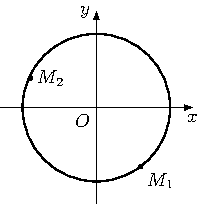
\includegraphics{2-1.pdf}
  \caption{}\label{fig:2-1}
\end{figurehere}
\end{minipage}

\begin{Practice}
  \begin{question}
    \item 到两坐标轴距离相等的点组成的直线的方程是 $x-y=0$ 吗? 为什么?
    \item 已知等腰三角形三个顶点的坐标是 $A\,(0,3)$,$B\,(-2,0)$,$C\,(2,0)$。中线 $AO$ 的方程是 $x=0$ 吗?为什么?
  \end{question}
\end{Practice}

\subsection{求曲线的方程}
我们先看两个例子。
\begin{example}
  设 $A$、$B$ 两点的坐标是 $(-1,-1)$、$(3,7)$,求线段 $AB$ 的垂直平分线的方程。
\end{example}
\noindent
\begin{minipage}{0.65\linewidth}\parindent2em
\begin{solution}
  设 $M\,(x,y)$ 是线段 $AB$ 的垂直平分线上任意一点(\cref{fig:2-2}),也就是点 $M$ 属于集合
  \[ P = \bigl\{ M \bigm\vert |MA|= |MB| \bigr\}. \]

  由两点的距离公式,点 $M$ 所适合的条件可表示为
  \[ \sqrt{(x+1)^2+(y+1)^2}=\sqrt{(x-3)^2+(y-7)^2}.\]
  两边平方后,得
\end{solution}
\end{minipage}\hfill
\begin{minipage}{0.3\linewidth}\centering
\begin{figurehere}
  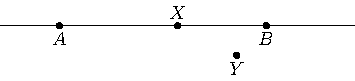
\includegraphics{2-2.pdf}
  \caption{}\label{fig:2-2}
\end{figurehere}
\end{minipage}

\medskip\noindent
\[(x+1)^2+(y+1)^2=(x-3)^2+(y-7)^2.\]
即
\begin{equation}
  \label{eq:mid_perp_line_equation}
  x+2y-7=0
\end{equation}

下面,我们证明\cref{eq:mid_perp_line_equation} 是线段 $AB$ 的垂直平分线的方程。
\begin{enumerate}[1 ]
  \item 由上面求方程的过程可知,垂直平分线上每一点的坐标都是\cref{eq:mid_perp_line_equation} 的解;
  \item 设点 $M_1$ 的坐标 $(x_1,y_1)$ 是方程\cref{eq:mid_perp_line_equation} 的解,即
  \begin{gather*}
    x_1+2y_1-7=0\\
    x_1=7-2y_1
  \end{gather*}
  点 $M_1$ 到 $A$、$B$ 的距离分别是
  \begin{align*}
    |M_1A| & = \sqrt{(x_1+1)^2+(y_1+1)^2}\\
           & = \sqrt{(8-2y_1)^2+(y_1+1)^2}\\
           & = \sqrt{5(y_1^2-6y_1+13)};
  \end{align*}
  \begin{align*}
    |M_1B| & = \sqrt{(x_1-3)^2+(y_1-7)^2}\\
           & = \sqrt{(4-2y_1)^2+(y_1-7)^2};\\
           & = \sqrt{5(y_1^2-6y_1+13)}.\\
    \therefore \quad |M_1A| & = |M_1B|,
  \end{align*}
  即点 $M_1$ 在线段 $AB$ 的垂直平分线上。
\end{enumerate}

由上述证明可知,方程\cref{eq:mid_perp_line_equation} 是线段 $AB$ 的垂直平分线的方程。

\medskip\noindent
\begin{minipage}{0.65\linewidth}\parindent2em
\begin{example}
  点 $M$ 与两条互相垂直的直线的距离的积是常数 $k$($k>0$),求点 $M$ 的轨迹方程。
\end{example}
\begin{solution}
  取已知两条互相垂直的直线为坐标轴,建立直角坐标系(\cref{fig:2-3})。

  设点 $M$ 的坐标为 $(x,y)$。点 $M$ 的轨迹就是与坐标轴的距离的积是常数 $k$ 的点的集合
  \[P = \bigl\{ M\bigm\vert |MR| \cdot |MQ|= k\bigr\},\]
  其中 $Q$、$R$ 分别是点 $M$ 到 $x$ 轴、$y$ 轴的垂线的垂足。
\end{solution}
\end{minipage}\hfill
\begin{minipage}{0.32\linewidth}\centering
  \begin{figurehere}
    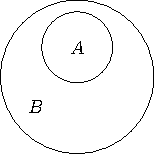
\includegraphics{2-3.pdf}
    \caption{}\label{fig:2-3}
  \end{figurehere}
\end{minipage}

\medskip
因为点 $M$ 到 $x$ 轴、 $y$ 轴的距离,分别是它的纵坐标和横坐标的绝对值,所以条件 $\left| {MR}\right| \cdot \left| {MQ}\right| = k$ 可写成
\[|x| \cdot |y| = k\]
即
\begin{equation}
\label{eq:inverse_proportion_equation} 
xy=\pm k.
\end{equation}
下面我们证明\cref{eq:inverse_proportion_equation} 是所求轨迹的方程。
\begin{enumerate}[1 ]
  \item\label{itm:proof_1} 由上面求方程的过程可知,曲线上的点的坐标都是\cref{eq:inverse_proportion_equation} 的解;
  \item\label{itm:proof_2} 设点 $M_1$ 的坐标 $(x_1,y_1)$ 是\cref{eq:inverse_proportion_equation} 的解,那么
  \[ x_1y_1=\pm k,\]
  即
  \[ |x_1|\cdot|y_1|=k.\]
  而 $|x_1|$、$|y_1|$ 正是点 $M_1$ 到纵轴、横轴的距离,因此点 $M_1$ 到这两条直线的距离的积是常数 $k$,点 $M_1$ 在\cref{eq:inverse_proportion_equation} 的曲线上。
\end{enumerate}

由~\ref{itm:proof_1}、\ref{itm:proof_2} 可知,\cref{eq:inverse_proportion_equation} 是所求轨迹的方程。图形如\cref{fig:2-3}。

由上面的例子可以看出,求曲线 (图形) 的方程,一般有下面几个步骤:
\begin{enumerate}
  \item\label{itm:proof_step1} 建立适当的直角坐标系,用 $(x,y)$ 表示曲线上任意一点 $M$ 的坐标;
  \item\label{itm:proof_step2} 写出适合条件 $p$ 的点 $M$ 的集合 $P = \{ M \mid p(M) \}$;
  \item\label{itm:proof_step3} 用坐标表示条件 $p(M)$ ,列出方程 $f(x,y)=0$;
  \item\label{itm:proof_step4} 化方程 $f(x,y)=0$ 为最简形式;
  \item\label{itm:proof_step5} 证明以化简后的方程的解为坐标的点都是曲线上的点。
\end{enumerate}

除个别情况外,化简过程都是同解变形过程,步骤~\ref{itm:proof_step5} 可以省略不写,如有特殊情况,可适当予以说明。
另外,根据情况,也可以省略步骤~\ref{itm:proof_step2},直接列出曲线方程。

\begin{example}
  已知一条曲线在 $x$ 轴的上方,它上面的每一点,到点 $A\,(0,2)$ 的距离减去它到 $x$ 轴的距离的差都是 2,求这条曲线的方程。
\end{example}
\noindent
\begin{minipage}{0.6\linewidth}\parindent2em
\begin{solution}
  设点 $M\,(x,y)$ 是曲线上任意一点,$MB \perp x$ 轴,垂足是 $B$(\cref{fig:2-4}),那么点 $M$ 属于集合
  \[P = \bigl\{ M\bigm||MA|-|MB|= 2\bigr\}\]
  由距离公式,点 $M$ 适合的条件可表示为
\end{solution}
\end{minipage}\hfill
\begin{minipage}{0.35\linewidth}\centering
  \begin{figurehere}
    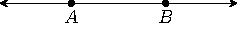
\includegraphics{2-4.pdf}
    \caption{}\label{fig:2-4}
  \end{figurehere}
\end{minipage}

\medskip
\begin{equation}
  \label{eq:parabolic_equation}
  \sqrt{x^2+(y-2)^2}-y=2.
\end{equation}
将\cref{eq:parabolic_equation} 移项后再两边平方,得
\[x^2+(y-2)^2 =(y+2)^2,\]
化简得:
\[y=\frac{1}{8}x^2.\]

因为曲线在 $x$ 轴的上方,$y>0$,虽然原点 $O$ 的坐标 $(0,0)$ 是这个方程的解,但不属于已知曲线,所以曲线的方程应是 $y=\dfrac{1}{8}x^2\,(x\neq 0)$,它的图形是关于 $y$ 轴对称的抛物线(\cref{fig:2-4}),但缺一个顶点。

求出曲线方程以后,我们就可以根据曲线的方程,来研究曲线的几何性质,这个问题,我们将在后面结合各种具体的曲线方程来说明。

\begin{Practice}
  \begin{question}
    \item 求到坐标原点的距离等于 2 的点的轨迹方程。
    \item 已知点 $M$ 与 $x$ 轴的距离和它与点 $F\,(0,4)$ 的距离相等,求点 $M$ 的轨迹方程。
  \end{question}
\end{Practice}

\subsection{充要条件}
从\cref{subsec:curve_equation}我们知道,$y=ax^2$ 是一条抛物线的方程。
这就是说,如果点 $M$ 的坐标是方程 $y=ax^2$ 的解,那么点 $M$ 一定是这条抛物线上的点。

象这样,我们就说“点 $M$ 的坐标是方程 $y=ax^2$ 的解”是“点 $M$ 在这条抛物线上”的充分条件。

又如,如果一个三角形有两个角相等,那么这个三角形是等腰三角形。

同样,我们说“有两个角相等”是“三角形是等腰三角形”的充分条件。

一般地,如果 $A$ 成立,那么 $B$ 成立,即 $A \to B$,这时我们就说条件 $A$ 是 $B$ 成立的充分条件。
也就是说,为使 $B$ 成立,具备条件 $A$ 就足够了。

再举一些充分条件的例子:
\begin{enumerate}
  \item 如果不重合的两条直线 $l_1$、$l_2$ 的斜率 $k_1=k_2$,那么 $l_1\parallel l_2$。因此,$k_1=k_2$ 是 $l_1\parallel l_2$ 的充分条件。
  \item 如果 $x=y$,那么 $x^2=y^2$。因此,$x=y$ 是 $x^2=y^2$ 的充分条件。
  \item 如果两个三角形全等,那么这两个三角形面积相等。因此,两个三角形全等是两个三角形面积相等的充分条件。
\end{enumerate}

从\cref{subsec:curve_equation}我们还知道,如果点 $M$ 在方程 $y=ax^2$ 的曲线上,那么点 $M$ 的坐标一定是方程 $y=ax^2$ 的解。

象这样,我们就说“点 $M$ 的坐标是方程 $y = a{x}^{2}$ 的解”是“点 $M$ 在抛物线上”的必要条件。

又如,如果三角形是等腰的,那么它有两个角相等。

同样,我们说“有两个角相等”是“三角形是等腰三角形”的必要条件。

一般地,如果 $B$ 成立,那么 $A$ 成立,即 $B \to A$,或者,如果 $A$ 不成立,那么 $B$ 就不成立,这时我们就说,条件 $A$ 是 $B$ 成立的必要条件。
也就是说,要使 $B$ 成立,就必须 $A$ 成立。
因为“$B \to A$ ”和它的逆否命题“$\bar{A} \to \bar{B}$”是等价的,所以,如果 $A$ 不成立,那么 $B$ 就一定不成立,也就是说,要使 $B$ 成立,$A$ 就必须成立。

再举一些必要条件的例子:
\begin{enumerate}
  \item 如果两条有斜率的直线 $l_1\parallel l_2$,那么它们的斜率 $k_1=k_2$,也就是,如果 $k_1\neq k_2$,那么 $l_1$ 与 $l_2$ 不平行。
  因此,$k_1=k_2$ 是 $l_1\parallel l_2$ 的必要条件。
  \item 如果 $x=y$ ,那么 $x^2=y^2$。也就是,如果 $x^2\neq y^2$,那么 $x\neq y$。因此,$x^2=y^2$ 是 $x=y$ 的必要条件。
  \item 如果两个三角形全等,那么这两个三角形的面积相等,也就是,如果两个三角形的面积不相等,那么它们不能全等。因此,两个三角形面积相等是它们全等的必要条件。
\end{enumerate}

综上所述,我们看到,如果 $A \to B$,那么 $A$ 是 $B$ 成立的充分条件;如果 $B \to A$,那么 $A$ 是 $B$ 成立的必要条件。

有时既有 $A \to B$,又有 $B \to A$,那么 $A$ 既是 $B$ 成立的充分条件,又是 $B$ 成立的必要条件。
这时,我们就说 $A$ 是 $B$ 成立的\Concept{充分而且必要的条件},简称\Concept{充要条件}。

例如,如果 $f(x,y)=0$ 是曲线 $C$ 的方程,那么“点 $M$ 的坐标是方程 $f(x,y)=0$ 的解”就是“点 $M$ 在曲线 $C$ 上” 的充要条件;“有两个角相等”就是“三角形是等腰三角形”的充要条件;“两条有斜率的直线 $l_1$、$l_2$ 的斜率 $k_1=k_2$”就是“$l_1\parallel l_2$”的充要条件。

应该注意,对于某个结论来说,有的条件是充分条件,但不是必要条件;也有的条件是必要条件,但不是充分条件。

例如,“$x=y$”是“$x^2=y^2$”的充分条件,但不是必要条件。因为要使 $x^2=y^2$,不一定要有 $x=y$,有 $x=-y$ 也可以了。

又如,两个三角形面积相等是它们全等的必要条件,但不是充分条件。因为得出两个三角形全等,只有面积相等是不够的。

充要条件是进一步学习时常用的数学概念之一。
\begin{Practice}
  \begin{question}
    \item “$b=0$”是“直线 $y=kx+b$ 过原点”的什么条件,为什么?
    \item “四边相等”是“一个四边形是正方形”的什么条件,为什么?
    \item “$x-1=0$”是“$x^2-1=0$”的什么条件,为什么?
    \item “两条直线不相交”是“这两条直线异面”的什么条件,为什么?
  \end{question}
\end{Practice}

\subsection{曲线的交点}
由曲线方程的定义可知,两条曲线交点的坐标应该是两个曲线方程的公共实数解,即两个曲线方程组成的方程组的实数解;反过来,方程组有几个实数解,两条曲线就有几个交点,方程组没有实数解,两条曲线就没有交点。
即两条曲线有交点的充要条件是它们的方程所组成的方程组有实数解。
可见,求曲线的交点的问题,就是求由它们的方程所组成的方程组的实数解的问题。

\begin{example}
  求直线 $y=x+\dfrac{3}{2}$ 被曲线 $y=\dfrac{1}{2}x^2$ 截得的线段的长。
\end{example}

\noindent
\begin{minipage}{0.6\linewidth}\parindent2em
\begin{solution}
  先求交点。

  解方程组
  \[ \begin{cases} y=x+\dfrac{3}{2},\\y=\dfrac{1}{2}x^2, \end{cases}\]
  得
  \[ \begin{cases} x_1=-1,\\y_1=\dfrac{1}{2}; \end{cases} \quad \begin{cases} x_2=3,\\ y_2=\dfrac{9}{2}.\end{cases}\]
\end{solution}
\end{minipage}\hfill
\begin{minipage}{0.35\linewidth}\centering
  \begin{figurehere}
    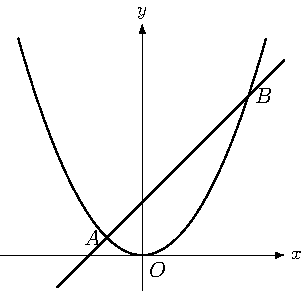
\includegraphics{2-5.pdf}
    \caption{}\label{fig:2-5}
  \end{figurehere}
\end{minipage}

\medskip\noindent
所以交点 $A$、$B$ 的坐标分别是 $\left(-1,\dfrac{1}{2}\right)$、$\left(3,\dfrac{9}{2}\right)$。直线被曲线截得的线段长
  \[|AB|=\sqrt{(3+1)^2+\left(\frac{9}{2}-\frac{1}{2}\right)^2}=4\sqrt{2}.\]

\begin{example}
  已知某圆的方程是 $x^2+y^2=2$。当 $b$ 为何值时,直线 $y=x+b$ 与圆有两个交点;两个交点重合为一点;没有交点?
\end{example}
\begin{solution}
  解方程组
  \begin{numcases}{}
    \label{eq:inter_line_equation} y=x+b,\\ \label{eq:circle_equation}x^2+y^2=2
  \end{numcases}
  把 \eqref{eq:inter_line_equation} 式代入 \eqref{eq:circle_equation} 式,得
  \begin{gather}
    x^2+(x+b)^2=2,\notag \\
    \label{eq:line_and_circle} 2x^2+2bx+b^2-2=0.
  \end{gather}
  \cref{eq:line_and_circle} 的根的判别式
  \[\begin{split} \Delta & = (2b)^2-4\times2(b^2-2) \\ &= 4(-b^2+4) \\ &=4(2+b)(2-b)\end{split}\]
\end{solution}

\medskip\noindent
\begin{minipage}{0.6\linewidth}\parindent2em
  当 $-2<b<2$ 时,$\Delta>0$,这时方程组有两个不同的实数解,因此直线与圆有两个交点;

  当 $b=-2$ 或 $b=2$ 时,$\Delta=0$,这时方程组有两个相同的实数解,因此直线与圆的两个交点重合为一点;

  当 $b>2$ 或 $b<-2$ 时,$\Delta<0$,这时方程组没有实数解,因此直线与圆没有交点。

  实际上,上述三种情况,就是直线与圆相交、相切、相离(\cref{fig:2-6})。
\end{minipage}\hfill
\begin{minipage}{0.35\linewidth}\centering
  \begin{figurehere}
    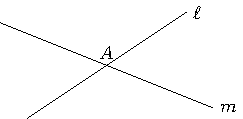
\includegraphics{2-6.pdf}
    \caption{}\label{fig:2-6}
  \end{figurehere}
\end{minipage}

\begin{Practice}
  求直线 $2x-5y+5=0$ 与曲线 $y=-\dfrac{10}{x}$ 的交点。
\end{Practice}

\begin{Exercise}
  \begin{question}
    \item 点 $A\,(1,-2)$、$B\,(2,-3)$、$C\,(3,10)$ 是否在方程
    \[ x^2-xy+2y+1=0\]
    的图形上?
    \item 解答:
    \begin{tasks}
      \task 在什么情况下,方程 $y=ax^2+bx+c$ 的曲线经过原点?
      \task 在什么情况下,方程 $(x-a)^2+(y-b)^2=r^2$ 的曲线经过原点?
    \end{tasks}
    \item 已知点 $M$ 到 $x$ 轴、$y$ 轴的距离的乘积等于 1。求点 $M$ 的轨迹方程。
    \item 点 $M$ 到点 $A\,(4,0)$ 和点 $B\,(-4,0)$ 的距离的和为 12,求点 $M$ 的轨迹方程。
    \item 一个点到点 $(4,0)$ 的距离等于它到 $y$ 轴的距离,求这个点的轨迹方程。
    \item 两个定点的距离为 6,点 $M$ 到这两个定点的距离的平方和为 26,求点 $M$ 的轨迹方程。
    \item 求与点 $O\,(0,0)$ 和 $A\,(c,0)$ 的距离的平方差为常数 $c$ 的点的轨迹方程。
    \item \label{exec:4-8}两根杆分别绕着定点 $A$ 和 $B$($AB=2a$)在平面内转动,并且转动时两杆保持相互垂直,求杆的交点 $P$ 的轨迹方程。
    \begin{figurehere}
      \begin{minipage}{\linewidth}\centering
        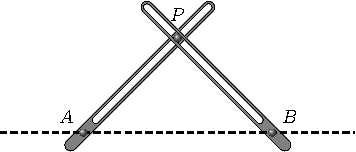
\includegraphics{ex4-8.pdf}
        \caption*{(第 \ref{exec:4-8} 题)}
      \end{minipage}
    \end{figurehere}
    \item 在下列横线上填写:“充分条件”或“必要条件”或“充要条件”:
    \begin{tasks}
      \task “$m$ 是有理数”是“$m$ 是实数”的\CJKunderline[hidden]{\quad 充分条件\quad };
      \task “$x^2-1=0$”是“$x-1=0$”的\CJKunderline[hidden]{\quad 必要条件\quad };
      \task “$x=2$”是“$x^2-5x+6=0$”的\CJKunderline[hidden]{\quad 充分条件\quad };
      \task “$x<5$”是“$x<3$”的\CJKunderline[hidden]{\quad 充分条件\quad };
      \task “内错角相等”是“二直线平行”的\CJKunderline[hidden]{\quad 充要条件\quad };
      \task “ABCD是矩形”是“ABCD是平行四边形”的\CJKunderline[hidden]{\quad 充分条件\quad };
      \task “两边和夹角对应相等”是“三角形全等”的\CJKunderline[hidden]{\quad 充要条件\quad }。
    \end{tasks}
    \item 求直线 $4x-3y=20$ 和圆 $x^2+y^2=25$ 的交点。
    \item 求经过两条曲线 $x^2+y^2+3x-y=0$ 和 $3x^2+3y^2+2x+y=0$ 交点的直线的方程。
  \end{question}
\end{Exercise}

\section{圆}
\subsection{圆的标准方程}
\medskip\noindent
\begin{minipage}{0.7\linewidth}\parindent2em
我们知道,平面内与定点距离等于定长的点的集合(轨迹)是圆。定点就是圆心,定长就是半径。

根据圆的定义,我们来求圆心是 $C(a,b)$,半径是 $r$ 的圆的方程(\cref{fig:2-7})。

设 $M\,(x,y)$ 是圆上任意一点,根据定义,点 $M$ 到圆心 $C$ 的距离等于 $r$。圆就是集合
\end{minipage}\hfill
\begin{minipage}{0.25\linewidth}\centering
\begin{figurehere}
  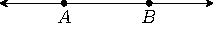
\includegraphics{2-7.pdf}
  \caption{}\label{fig:2-7}
\end{figurehere}
\end{minipage}

\[ P=\bigl\{ M \bigm\vert |MC|=r \bigr\}.\]

由两点的距离公式,点 $M$ 适合的条件可表示为
\begin{equation}
  \label{eq:circle_point_distance}
  \sqrt{(x-a)^2+(y-b)^2}=r.
\end{equation}

把\cref{eq:circle_point_distance} 两边平方,得
\begin{equation}
  \label{eq:standard_circle_equation}
  \tcbhighmath{(x-a)^2+(y-b)^2=r^2}.
\end{equation}

\cref{eq:standard_circle_equation} 就是圆心是 $C\,(a,b)$,半径是 $r$ 的圆的方程。
我们把它叫做\Concept{圆的标准方程}。 

如果圆心在坐标原点,这时 $a=0$,$b=0$,那么圆的方程就是
\[ x^2+y^2=r^2.\]

\begin{example}
  已知两点 $P_1\,(4,9)$ 和 $P_2\,(6,3)$,求以 $P_1P_2$ 为直径的圆的方程,并且判断点 $M\,(6,9)$、$N\,(3,3)$、$Q\,(5,3)$ 是在圆上,在圆内,还是在圆外。
\end{example}
\begin{solution}
根据已知条件,圆心 $C\,(a,b)$ 是 $P_1P_2$ 的中点,那么它的坐标为
\[ a=\frac{4+6}{2}=5,\quad b = \frac{9+3}{2}=6.\]

再根据两点的距离公式,得圆的半径是
\[r=|CP_1|=\sqrt{(4-5)^2+(9-6)^2} =\sqrt{10}.\]
因此所求圆的方程是
\[(x-5)^2+(y-6)^2=10.\]

分别计算点 $M\,(6,9)$、$N\,(3,3)$、$Q\,(5,3)$ 与圆心 $C\,(5,6)$ 的距离,得
\begin{gather*}
  |CM|=\sqrt{(6-5)^2+(9-6)^2}=\sqrt{10},\\
  |CN|=\sqrt{(3-5)^2+(3-6)^2}=\sqrt{13}>\sqrt{10},\\
  |CQ|=\sqrt{(5-5)^2+(3-6)^2}=3<\sqrt{10},
\end{gather*}
因此,点 $M$ 在圆上,点 $N$ 在圆外,点 $Q$ 在圆内。
\end{solution}

\begin{example}
求以 $C\,(1,3)$ 为圆心,并且和直线 $3x-4y-7=0$ 相切的圆的方程。
\end{example}
\begin{solution}
  已知圆心是 $C\,(1,3)$,那么只要再求出圆的半径 $r$,就能写出圆的方程。

  因为圆 $C$ 和直线 $3x-4y-7=0$ 相切,所以半径 $r$ 等于圆心 $C$ 到这条直线的距离。根据点到直线的距离公式,得
  \[r=\frac{|3\times 1-4\times 3-7|}{\sqrt{3^2+(-4)^2}}=\frac{16}{5}.\]
  因此,所求的圆的方程是
  \[(x-1)^2+(y-3)^2=\frac{256}{25}.\]
\end{solution}

\begin{example}
  已知圆的方程是 $x^2+y^2=r^2$ ,求经过圆上一点 $M\,(x_0,y_0)$ 的切线的方程。
\end{example}
\noindent
\begin{minipage}{0.68\linewidth}\parindent2em
\begin{solution}
  如\cref{fig:2-8},设切线的斜率为 $k$,半径 $OM$ 的斜率为 $k_1$。因为圆的切线垂直于过切点的半径,于是 $k=-\dfrac{1}{k_1}$。
  \begin{gather*}
    \because \quad k_1=\frac{y_0}{x_0}\\
    \therefore \quad k=-\frac{x_0}{y_0}
  \end{gather*}
\end{solution}
\end{minipage}\hfill
\begin{minipage}{0.27\linewidth}\centering
\begin{figurehere}
  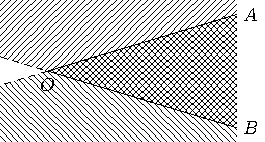
\includegraphics{2-8.pdf}
  \caption{}\label{fig:2-8}
\end{figurehere}
\end{minipage}

\medskip\noindent
经过点 $M$ 的切线方程是
  \[y-y_0=-\frac{x_0}{y_0}(x-x_0),\]
  整理得
  \[ x_0x+y_0y=x_0^2+y_0^2,\]
  因为点 $M\,(x_0,y_0)$ 在圆上,所以 $x_0^2+y_0^2=r^2$,所求切线方程是
  \[x_0x+y_0y=r^2.\]
\begin{example}
  \cref{fig:2-9} 是某圆拱桥的一孔圆拱的示意图。该圆拱跨度 $AB=\qty{20}{m}$,拱高 $OP=\qty{4}{m}$,在建造时每隔 \qty{4}{m} 需用一个支柱支撑,求支柱 $A_2P_2$ 的长度(精确到 \qty{0.01}{m})。
\end{example}
\noindent
\begin{minipage}{0.5\linewidth}\parindent2em
\begin{solution}
建立坐标系如\cref{fig:2-9}。圆心在 $y$ 轴上。设圆心的坐标是 $(0,b)$,圆的半径是 $r$,那么圆的方程是
\[x^2+(y-b)^2=r^2.\]
\end{solution}
\end{minipage}\hfill
\begin{minipage}{0.45\linewidth}\centering
  \begin{figurehere}
    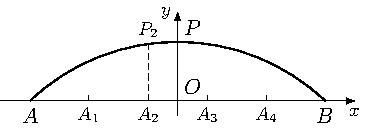
\includegraphics{2-9.pdf}
    \caption{}\label{fig:2-9}
  \end{figurehere}
\end{minipage}

\medskip
下面用待定系数法来确定 $b$ 和 $r$ 的值。

因为 $P$、$B$ 都在圆上,所以它们的坐标 $(0,4)$、$(10,0)$ 都是这个圆的方程的解。于是得到方程组:
\[\begin{cases} 0^2+(4-b)^2=r^2,\\10^2+(0-b)^2=r^2. \end{cases}\]
解得
\[b=-10.5,\quad r^2=14.5^2.\]

$\therefore\ $ 这个圆的方程是
\[ x^2+(y+10.5)^2=14.5^2.\]

把点 $P_2$ 的横坐标 $x=-2$ 代入这个圆的方程,得
\begin{gather*}
  (-2)^2+(y+10.5)^2=14.5^2,\\
  y+10.5=\sqrt{14.5^2-(-2)^2},
\end{gather*}
(因为 $P_2$ 的纵坐标 $y>0$,所以方根取正值。)
\begin{align*}
  y&= \sqrt{14.5^2-(-2)^2} -10.5\\
  &\approx 14.36-10.5 \\
  &= \qty{3.86}{m}.
\end{align*}
答:支柱 $A_2P_2$ 的长度约为 \qty{3.86}{m}。

\begin{Practice}
  \begin{question}
    \item 写出下列各圆的方程:
    \begin{tasks}
      \task 圆心在原点,半径是 3;
      \task 圆心在点 $C\,(3,4,)$,半径是 $\sqrt{5}$;
      \task 经过点 $P\,(5,1)$,圆心在点 $C\,(8,-3)$。
    \end{tasks}
    \item 一个圆过点 $P\,(12,0)$,且与 $y$ 轴切于原点。求这个圆的方程,并判断点 $A\,(6,-6)$、$B\,(5,-5)$、$C\,(2.5,5)$ 是在圆内,在圆外,还是在圆上。
    \item 已知一个圆的圆心在原点,并与直线 $4x+3y-70=0$ 相切。求圆的方程。
    \item 写出过圆 $x^2+y^2=10$ 上一点 $M\,(2,\sqrt{6})$ 的切线的方程。
    \item 已知圆的方程是 $x^2+y^2=1$。求:
    \begin{tasks}
      \task 斜率等于 1 的切线方程;
      \task 在 $y$ 轴上截距是 $\sqrt{2}$ 的切线方程。
    \end{tasks}
  \end{question}
\end{Practice}

\subsection{圆的一般方程}
把圆的标准方程
\[(x-a)^2+(y-b)^2=r^2\]
展开,得
\[x^2+y^2-2ax-2by+a^2+b^2-r^2=0.\]
可见,任何一个圆的方程都可以写成下面的形式:
\begin{equation}
  \label{eq:circle_general_equation}
  \tcbhighmath{x^2+y^2+Dx+Ey+F=0}.
\end{equation}

反过来,我们来研究形如\cref{eq:circle_general_equation} 的方程的曲线是不是圆。

将\cref{eq:circle_general_equation} 的左边配方,得
\begin{equation}
  \label{eq:circle_general_standard_equation}
  \left(x+\frac{D}{2}\right)^2+\left(y+\frac{E}{2}\right)^2=\frac{D^2+E^2-4F}{4}.
\end{equation}
\begin{enumerate}[1.,itemsep=5pt]
  \item 当 $D^2+E^2-4F>0$ 时,比较\cref{eq:circle_general_standard_equation} 和圆的标准方程,可以看出\cref{eq:circle_general_equation} 表示以 $\left(-\dfrac{D}{2},-\dfrac{E}{2}\right)$ 为圆心、$\dfrac{1}{2}\sqrt{D^2+E^2-4F}$ 为半径的圆;
  \item 当 $D^2+E^2-4F=0$ 时,\cref{eq:circle_general_equation} 只有实数解 $x=-\dfrac{D}{2}$、$y=-\dfrac{E}{2}$,所以表示一个点 $\left(-\dfrac{D}{2},-\dfrac{E}{2}\right)$;
  \item 当 $D^2+E^2-4F<0$ 时,\cref{eq:circle_general_equation} 没有实数解,因而它不表示任何图形。
\end{enumerate}

因此,当 $D^2+E^2-4F>0$ 时,\cref{eq:circle_general_equation} 表示一个圆,\cref{eq:circle_general_equation} 叫做\Concept{圆的一般方程}。

圆的标准方程的优点在于它明确地指出了圆心和半径,而一般方程突出了方程形式上的特点:
\begin{enumerate}
  \item $x^2$ 和 $y^2$ 的系数相同,不等于零;
  \item 没有 $xy$ 这样的二次项。
\end{enumerate}

以上两点是二元二次方程
\[ Ax^2+Bxy+Cy^2+Dx+Ey+F=0\]
表示圆的必要条件,但不是充分条件。

要求圆的一般方程,只要求出三个系数 $D$、$E$、$F$ 就可以了。
\begin{example}
  求过三点 $O\,(0,0)$、$M_1\,(1,1)$、$M_2\,(4,2)$ 的圆的方程,并求这个圆的半径和圆心坐标。
\end{example}

\begin{solution}
  设所求的圆的方程为
  \[ x^2+y^2+Dx+Ey+F=0 \]
  用待定系数法,根据所给条件,来确定 $D$、$E$、$F$。

  因 $O$、$M_1$、$M_2$ 在圆上,所以它们的坐标是方程的解。把它们的坐标依次代入上面的方程,得到关于 $D$、$E$、$F$ 的三元一次方程组:
  \[\begin{cases} F=0,\\D+E+F+2=0,\\4D+2E+F+20=0. \end{cases}\]
  解这个方程组,得 $F=0$,$D=-8$,$E=6$。于是得到所求圆的方程
  \[x^2+y^2-8x+6y=0\]

  由前面的讨论可知,圆的半径 $r=\dfrac{1}{2}\sqrt{D^2+E^2-4F}=5$,圆心坐标是 $(4,-3)$。
\end{solution}
\begin{example}
  已知一曲线是与两个定点 $O\,(0,0)$、$A\,(3,0)$ 距离的比为 $\dfrac{1}{2}$ 的点的轨迹,求这个曲线的方程,并画出曲线。
\end{example}
\noindent
\begin{minipage}{0.6\linewidth}\parindent2em
\begin{solution}
  在给定的坐标系里,设点 $M\,(x,y)$ 是曲线上的任意一点,也就是点 $M$ 属于集合
  \[P=\left\{ M \middle\vert \frac{|OA|}{|AM|}=\frac{1}{2} \right\}.\]

  由两点的距离公式,点 $M$ 所适合的条件可以表示为
\end{solution}
\end{minipage}\hfill
\begin{minipage}{0.35\linewidth}\centering
\begin{figurehere}
  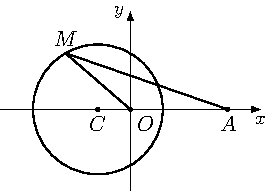
\includegraphics{2-10.pdf}
  \caption{}\label{fig:2-10}
\end{figurehere}
\end{minipage}

\medskip
\begin{equation}
  \label{eq:equal_distance_M}
  \frac{\sqrt{x^2+y^2}}{\sqrt{(x-3)^2+y^2}}=\frac{1}{2}.
\end{equation}
将\cref{eq:equal_distance_M} 两边平方,得
\[ \frac{x^2+y^2}{(x-3)^2+y^2}=\frac{1}{4}\]
化简得
\begin{equation}
  \label{eq:M_trace}
  x^2+y^2+2x-3=0
\end{equation}
这就是所求的曲线方程。

把\cref{eq:M_trace} 配方,得
\[ (x+1)^2+y^2=4\]
所以\cref{eq:M_trace} 的曲线是以 $C\,(-1,0)$ 为圆心,$r=2$ 为半径的圆,它的图形如\cref{fig:2-10}。

\begin{Practice}
  \begin{question}
    \item 下列方程各表示什么图形?
    \begin{tasks}(2)
      \task $x^2+y^2=0$;
      \task $x^2+y^2-2x+4y-6=0$;
      \task $x^2+y^2+2ax-b^2=0$。
    \end{tasks}
    \item 求下列各圆的半径和圆心坐标:
    \begin{tasks}(2)
      \task $x^2+y^2-6x=$;
      \task $x^2+y^2+2by=0$。
    \end{tasks}
  \end{question}
\end{Practice}

\begin{Exercise}
  \begin{question}
    \item 求下列各圆的方程,并画出它的图形:
    \begin{tasks}
      \task 过点 $C\,(-1,1)$ 和 $D\,(1,3)$,圆心在 $x$ 轴上;
      \task 过直线 $x+3y+7=0$ 与 $3x-2y-12=0$ 的交点,圆心为点 $C\,(-1,1)$;
      \task 半径是 5,圆心在 $y$ 轴上,且与直线 $y=6$ 相切;
      \task 过点 $A\,(5,2)$ 和 $B\,(3,-2)$,圆心在直线 $2x-y=3$ 上。
    \end{tasks}
    \item 求下列条件所决定的圆的方程:
    \begin{tasks}
      \task 圆心为 $C\,(3,-5)$,并且与直线 $x-7y+2=0$ 相切;
      \task 过点 $A\,(3,2)$,圆心在直线 $y=2x$ 上,且与直线 $y=2x+5$ 相切。
    \end{tasks}
    \item 已知: 一个圆的直径端点是 $A\,(x_1,y_1)$、$B\,(x_2,y_2)$。证明:圆的方程是 $(x-x_1)(x-x_2)+(y-y_1)(y-y_2)=0$。
    \item 一个等腰三角形底边上的高等于 5,底边两端点的坐标是 $(-4,0)$ 和 $(4,0)$ 。求它的外接圆的方程。
    \item 赵州桥的跨度是 \qty{37.4}{m},圆拱高约为 \qty{7.2}{m}。求这座圆拱桥的拱圆的方程。
    \item 求通过点 $A,(1,2)$,且与两坐标轴同时相切的圆的方程。
    \item 过点 $A\,(0,\sqrt{10})$ 向圆 $x^2+y^2=5$ 引两条切线。求它们的方程。
    \item 求下列各圆的一般方程:
    \begin{tasks}
      \task 过点 $A\,(5,1)$,圆心在点 $C\,(8,-3)$;
      \task 过三点 $A\,(-1,5)$、$B\,(5,5)$、$C\,(6,-2)$。
    \end{tasks}
    \item \label{exec:5-9}某工件尺寸如图所示,它的外缘由四段圆弧连接而成。求各段圆弧所在的圆的方程。
    \begin{figurehere}
      \begin{minipage}{\linewidth}\centering
        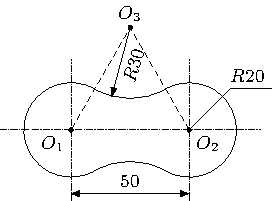
\includegraphics{ex5-9.pdf}
        \caption*{(第 \ref{exec:5-9} 题)}
      \end{minipage}
    \end{figurehere}
    \item 求下列各圆的圆心坐标和半径,并画出它们的图形:
    \begin{tasks}(2)
      \task $x^2+y^2-2x-5=0$;
      \task $x^2+y^2+2x-4y-4=0$;
      \task $x^2+y^2+2ax=0$ ;
      \task $x^2+y^2-2by-2b^2=0$。
    \end{tasks}
    \item 求证:两圆 $x^2+y^2-4x-6y+9=0$ 和 $x^2+y^2+12x+6y-19=0$ 相外切。
    \item 求直线 $4x-3y=50$ 和圆 $x^2+y^2=100$ 的交点,说明它们的位置关系。
    \item 求经过两圆 $x^2+y^2+6x-4=0$ 和 $x^2+y^2+6y-28=0$ 的交点,并且圆心在直线 $x-y-4=0$ 上的圆的方程。
    \item 等腰三角形的顶点是 $A\,(4,2)$,底边一个端点是 $B\,(3,5)$。求另一个端点的轨迹方程,并说明它的轨迹是什么。
    \item 一条线段 $AB$($AB=2a$)的两个端点 $A$ 和 $B$ 分别在 $x$ 轴和 $y$ 轴上滑动。求线段 $AB$ 的中点 $M$ 的轨迹方程。
  \end{question}
\end{Exercise}

\section{椭圆}
\subsection{椭圆及其标准方程}
\medskip\noindent
\begin{minipage}{0.5\linewidth}\parindent2em
椭圆是一种常见的曲线,如汽车油罐横截面的轮廓,天体中一些行星和卫星运行的轨道。
在立体几何中画直观图时,圆的一种直观图也是椭圆。

取一条一定长的细绳,把它的两端固定在画图板上的 $F_1$ 和 $F_2$ 两点(\cref{fig:2-11}),当绳长大于 $F_1$ 和 $F_2$ 的距离时,用铅笔尖
\end{minipage}\hfill
\begin{minipage}{0.45\linewidth}\centering
\begin{figurehere}
  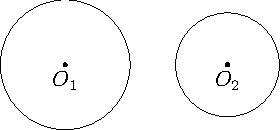
\includegraphics{2-11.pdf}
  \caption{}\label{fig:2-11}
\end{figurehere}
\end{minipage}

\medskip\noindent
把绳子拉紧,使笔尖在图板上慢慢移动,就可以画出一个椭圆。

从上面的画图过程,我们可以看出,椭圆是由与点 $F_1$ 和 $F_2$ 的距离的和等于这条绳长的点组成的。

我们把平面内与两个定点 $F_1$、$F_2$ 的距离的和等于常数(大于 $|F_1F_2|$)的点的轨迹叫做\Concept{椭圆}。
这两个定点叫做椭圆的\Concept{焦点},两焦点的距离叫做\Concept{焦距}。

\medskip\noindent
\begin{minipage}{0.6\linewidth}\parindent2em
根据椭圆的定义,我们来求椭圆的方程。

取过焦点 $F_1$、$F_2$ 的直线为 $x$ 轴,线段 $F_1F_2$ 的垂直平分线为 $y$ 轴,建立直角坐标系(\cref{fig:2-12})。

设 $M\,(x,y)$ 是椭圆上任意一点,椭圆的焦距为 $2c$($c>0$),$M$ 与 $F_1$ 和 $F_2$ 的距离的和等于正常数 $2a$,则 $F_1$、$F_2$ 的坐标分别是 $(-c,0)$、$(c,0)$。
\end{minipage}\hfill
\begin{minipage}{0.35\linewidth}\centering
\begin{figurehere}
  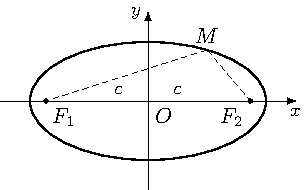
\includegraphics{2-12.pdf}
  \caption{}\label{fig:2-12}
\end{figurehere}
\end{minipage}

\medskip
椭圆就是集合
\[P=\bigr\{M \bigm\vert |MF_1|+|MF_2|=2a \bigr\}.\]
\[ \because \quad |MF_1|=\sqrt{(x+c)^2+y^2},|MF_2|=\sqrt{(x-c)^2+y^2},\]
得方程
\[\sqrt{(x+c)^2+y^2}+\sqrt{(x-c)^2+y^2}=2a.\]
将这个方程移项,两边平方,得
\begin{gather*}
  (x+c)^2+y^2=4a^2-4a\sqrt{(x-c)^2+y^2}+(x-c)^2+y^2,\\
  a^2-cx=a\sqrt{(x-c)^2+y^2}.
\end{gather*}
两边再平方,得
\[a^4-2a^2cx+c^2x^2=a^2x^2-2a^2cx+a^2c^2+a^2y^2,\]
整理得
\[(a^2-c^2)x^2+a^2y^2=a^2(a^2-c^2).\]

由椭圆定义可知,$2a>2c$,即 $a>c$,所以 $a^2-c^2>0$。

设 $a^2-c^2=b^2$($b>0$),得
\[ b^2x^2+a^2y^2=a^2b^2,\]
两边除以 $a^2b^2$,得
\begin{equation}
  \label{eq:ellipse_standard_equation} 
  \tcbhighmath{\frac{x^2}{a^2}+\frac{y^2}{b^2}=1\quad(a>b>0)}.
\end{equation}


\medskip\noindent
\begin{minipage}{0.6\linewidth}\parindent2em
这个方程叫做\Concept{椭圆的标准方程}。
它所表示的椭圆的焦点在 $x$ 轴上,焦点是 $F_1\,(-c,0)$、$F_2\,(c,0)$,这里 $c^2=a^2-b^2$。

如果椭圆的焦点在 $y$ 轴上,焦点是 $F_1\,(0,-c)$、$F_2\,(0,c)$(\cref{fig:2-13}),只要将\cref{eq:ellipse_standard_equation} 的 $x$、$y$ 互换,就可以得到它的方程。这时方程为
\[ \frac{y^2}{a^2}+\frac{x^2}{b^2}=1\quad(a>b>0). \]
这个方程也是椭圆的标准方程。
\end{minipage}\hfill
\begin{minipage}{0.35\linewidth}\centering
\begin{figurehere}
  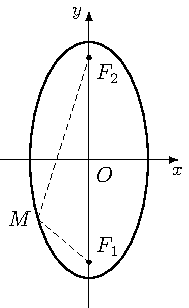
\includegraphics{2-13.pdf}
  \caption{}\label{fig:2-13}
\end{figurehere}
\end{minipage}

\medskip
\begin{example}
  平面内两个定点的距离是 8,写出到这两个定点的距离的和是 10 的点的轨迹的方程。
\end{example}
\begin{solution}
  这个轨迹是一个椭圆,两个定点是焦点,用 $F_1$、$F_2$ 表示。取过点 $F_1$ 和 $F_2$ 的直线为 $x$ 轴,线段 $F_1F_2$ 的垂直平分线为 $y$ 轴。
\begin{gather*}
  \because\quad  2a=10,\quad 2c=8.\\
  \therefore\quad a=5,\quad c=4.\\
  b^2=a^2-c^2=5^2-4^2=9,\quad b=3.
\end{gather*}
因此,这个椭圆的标准方程是
\[ \frac{x^2}{5^2}+\frac{y^2}{3^2}=1\quad \text{即} \quad \frac{x^2}{25}+\frac{y^2}{9}=1.\]

如果取过 $F_1$ 和 $F_2$ 的直线为 $y$ 轴,线段 $F_1F_2$ 的垂直平分线为 $x$ 轴,则这个椭圆的标准方程是
\[ \frac{y^2}{25}+\frac{x^2}{9}=1.\]
\end{solution}

\begin{example}\label{exam:drawing_ellipse}
  已知椭圆焦距是 $2c$,用直尺和圆规作点画出与两个焦点距离的和是 $2a$ 的椭圆。
\end{example}
\begin{solution}
  \begin{enumerate}
    \item 作线段 $F_1F_2$,使 $|F_1F_2|=2c$。设 $F_1F_2$ 的中点为 $O$,在 $F_1F_2$ 和 $F_2F_1$ 的延长线上,分别取点 $A$、$A'$;使 $OA=OA'=a$(\cref{fig:2-14})。
  \end{enumerate}

  \medskip\noindent
  \begin{minipage}{0.6\linewidth}\parindent2em
  \begin{enumerate}[resume]
    \item 在线段 $F_1F_2$ 上任取一点 $M_1$,分别以点 $F_1$、$F_2$ 为圆心,$A'M_1$、$AM_1$ 为半径画弧,交于点 $P_1$、$P'_1$。改变 $M_1$ 的位置,例如 $M_2,M_3,\cdots$,用同样方法作出点 $P_2$、$P'_2$、$P_2$、$P'_2$……。
    \item 把 $A‘$、$P_1$、$P2$、$\cdots$、$A$、$\cdots$、$P'_2$、$P'_1$、$A'$ 顺次连成光滑曲线,就得到所求的椭圆。
  \end{enumerate}
\end{minipage}\hfill
  \begin{minipage}{0.35\linewidth}\centering
    \begin{figurehere}
      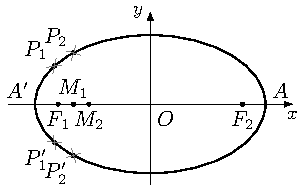
\includegraphics{2-14.pdf}
      \caption{}\label{fig:2-14}
    \end{figurehere}
  \end{minipage}

  % \medskip
  % \begin{enumerate}[resume]  
  %   \item 把 $A‘$、$P_1$、$P2$、$\cdots$、$A$、$\cdots$、$P'_2$、$P'_1$、$A'$ 顺次连成光滑曲线,就得到所求的椭圆。
  % \end{enumerate}
\end{solution}
\begin{Practice}
  \begin{question}
    \item 说明\cref{exam:drawing_ellipse} 中椭圆画法的依据。
    \item 写出适合下列条件的椭圆的标准方程:
    \begin{tasks}
      \task $a=4,b=1$,焦点在 $x$ 轴上;
      \task $a=4,c=\sqrt{15}$,焦点在 $y$ 轴上;
      \task 两个焦点的坐标是 $(-2,0)$ 和 $(2,0)$,并且经过点$(\dfrac{5}{2},- \dfrac{3}{2})$。
    \end{tasks}
    \item 已知 $\triangle ABC$ 的一边 $BC$ 长为 6,周长为 16。求顶点 $A$ 的轨迹方程。
  \end{question}
\end{Practice}

\subsection{椭圆的几何性质}
我们根据椭圆的标准方程
\[\frac{x^2}{a^2}+\frac{y^2}{b^2}=1 \quad(a>b>0)\]
来研究椭圆的几何性质。
\subsubsection{范围}
由标准方程可知,椭圆上点的坐标 $(x,y)$ 都适合不等式
\[ \frac{x^2}{a^2}\leqslant 1, \frac{y^2}{b^2}\leqslant 1, \]
\begin{minipage}{0.55\linewidth}
即
\begin{gather*} 
  x^2\leqslant a^2,\quad y^2\leqslant b^2,\\
  \therefore\quad |x|\leqslant|a|, |y|\leqslant|b|.
\end{gather*}
这说明椭圆位于直线 $x=\pm a$ 和 $y=\pm b$ 所围成的矩形里(\cref{fig:2-15})。
\end{minipage}\hfill
\begin{minipage}{0.4\linewidth}\centering
\begin{figurehere}
  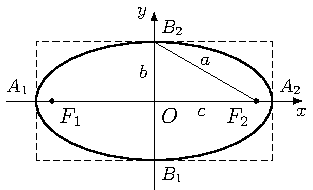
\includegraphics{2-15.pdf}
  \caption{}\label{fig:2-15}
\end{figurehere}
\end{minipage}

\subsubsection{对称性}
在标准方程中,把 $x$ 换成 $-x$;或把 $y$ 换成 $-y$;或把 $x$、$y$ 同时换成 $-x$、$-y$ 时,方程都不变。所以图形关于 $y$ 轴、$x$ 轴和原点都是对称的。这时,坐标轴是椭圆的对称轴,原点是椭圆的对称中心。椭圆的对称中心叫做椭圆的\Concept{中心}。

\subsubsection{顶点}
在标准方程中,令 $x=0$,得 $y=\pm b$。这说明 $B_1\,(0,-b)$、$B_2\,(0,b)$ 是椭圆和 $y$ 轴的两个交点。同理,令 $y=0$ 时,得 $x=\pm a$,$A_1\,(-a,0)$、$A_2\,(a,0)$ 是椭圆和 $x$ 轴的两个交点。因为 $x$ 轴、$y$ 轴是椭圆的对称轴,所以椭圆和它的对称轴有四个交点,这四个交点,叫做椭圆的\Concept{顶点}。

线段 $A_1A_2$、$B_1B_2$ 分别叫做椭圆的\Concept{长轴}和\Concept{短轴}。它们的长分别等于 $2a$ 和 $2b$,$a$ 和 $b$ 分别叫做椭圆的长半轴长和短半轴长。

\subsubsection{离心率}
椭圆的焦距与长轴长的比 $e=\dfrac{c}{a}$,叫做椭圆的\Concept{离心率}。

因为 $a>c>0$,所以 $0<e<1$。$e$ 越接近 1,则 $c$ 越接近 $a$,从而 $b=\sqrt{a^2-c^2}$ 越小,因此椭圆越扁;反之,$e$ 越接近于 0,$c$ 越接近于 0,从而 $b$ 越接近于 $a$,这时椭圆就接近于圆。

如果 $a=b$,则 $c=0$,两个焦点重合,这时椭圆的标准方程成为
\[x^2+y^2=a^2\]
图形就是圆了。

\begin{example}
求椭圆 $16x^2+25y^2=400$ 的长轴和短轴的长、离心率、焦点和顶点的坐标,并用描点法画出它的图形。
\end{example}
\begin{solution}
  把已知方程化成标准方程
  \[ \frac{x^2}{5^2}+\frac{y^2}{4^2}=1\]
  这里,$a=5$,$b=4$,$c=\sqrt{25-16}=3$。

  因此,椭圆的长轴和短轴的长分别是 $2a=10$ 和 $2b=8$,离心率 $e=\dfrac{c}{a}= \dfrac{3}{5}={0.6}$,两个焦点分别是 $F_1\,(-3,0)$ 和 $F_2\,(3,0)$,椭圆的四个顶点是 $A_1\,(-5,0)$、$A_2\,(5,0)$、$B_1\,(0,-4)$ 和 $B_2\,(0,4)$。

  将已知方程变形为 $y=\pm\dfrac{4}{5}\sqrt{25-x^2}$。根据
  \[y=+\frac{4}{5}\sqrt{25-x^2},\]
  在第一象限 $x\leqslant 5$ 的范围内算出几个点的坐标 $(x,y)$:
  \begin{tablehere}
    \begin{tblr}{colspec={*7{X[c]}},vline{2}={0.8pt}}
      $x$ & 0 & 1 & 2 & 3 & 4 & 5 \\
      $y$ & 4 & 3.9 & 3.7 & 3.2 & 2.4 & 0 \\
    \end{tblr}
  \end{tablehere}
  
  先描点画出椭圆在第一象限内的图形,再利用椭圆的对称性就画出整个椭圆(\cref{fig:2-16})。
\end{solution}
\begin{figure}
  \begin{minipage}[b]{0.48\linewidth}\centering
    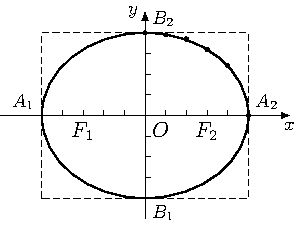
\includegraphics{2-16.pdf}
    \caption{}\label{fig:2-16}
  \end{minipage}
  \begin{minipage}[b]{0.48\linewidth}\centering
    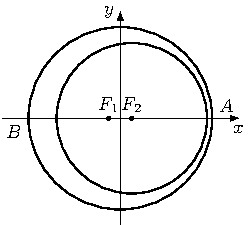
\includegraphics{2-17.pdf}
    \caption{}\label{fig:2-17}
  \end{minipage}
\end{figure}

\begin{example}
我国发射的第一颗人造地球卫星的运行轨道,是以地球的中心为一个焦点的椭圆,近地点 $A$ 距地面 \qty{439}{km},远地点 $B$ 距地面 \qty{2384}{km},地球半径约为 \qty{6371}{km}。求卫星的轨道方程。
\end{example}
\begin{solution}
  选取坐标系如\cref{fig:2-17}。
  \begin{gather*}
    a-c=|OA|-|OF_2|=|F_2A|=6371+439=6810,\\
    a+c=|OB|+|OF_2|=|F_2B|=6371+2384=8755.
  \end{gather*}
  解得
  \begin{gather*}
    a=7782.5,\quad c=972.5.\\
    \therefore \quad b=\sqrt{a^2-c^2} = \sqrt{(a+c)(a-c)} = \sqrt{8755\times 6810}= 7211.5
  \end{gather*}
  因此,卫星的轨道方程(近似)是
  \[ \frac{x^2}{7783^2}+\frac{y^2}{7722^2} = 1.\]
\end{solution}

\begin{example}
  点 $M\,(x,y)$ 与定点 $F\,(c,0)$ 的距离和它到定直线 $l:x=\dfrac{a^2}{c}$ 的距离的比是常数 $\dfrac{c}{a}$($a>c>0$)。求点 $M$ 的轨迹(\cref{fig:2-18})。
\end{example}

\noindent
\begin{minipage}{0.55\linewidth}\parindent2em
\begin{solution}
  设 $d$ 是点 $M$ 到直线 $l$ 的距离。根据题意,所求轨迹就是集合
  \[P=\left\{ M \middle\vert \frac{|MF|}{d}=\frac{c}{a} \right\}.\]
  由此得
  \[\frac{\sqrt{(x-c)^2+y^2}}{\left|\dfrac{a^2}{c}-x\right|}=\frac{c}{a}.\]
\end{solution}
\end{minipage}\hfill
\begin{minipage}{0.4\linewidth}\centering
  \begin{figurehere}
    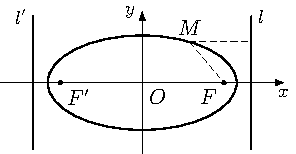
\includegraphics{2-18.pdf}
    \caption{}\label{fig:2-18}
  \end{figurehere}
\end{minipage}

\medskip\noindent
将上式化简,得
  \[(a^2-c^2)x^2+a^2y^2=a^2(a^2-c^2).\]

  设 $a^2-c^2=b^2$,就可化成
  \[ \frac{x^2}{a^2}+\frac{y^2}{b^2}=1\]
这是椭圆的标准方程,所以点 $M$ 的轨迹是椭圆。

由上面的例子可知,点 $M$ 与一个定点的距离和它到一条定直线的距离的比是常数 $e= \dfrac{c}{a}$($e<1$)时,这个点的轨迹是椭圆。
定点是椭圆的焦点,定直线叫做椭圆的\Concept{准线},常数 $e$ 是椭圆的离心率。

对于椭圆 $\dfrac{x^2}{a^2}+\dfrac{y^2}{b^2}=1$,相应于焦点 $F\,(c,0)$ 的准线方程是 $x=\dfrac{a^2}{c}$。根据椭圆的对称性,相应于焦点 $F'\,(-c,0)$ 的准线方程是 $x=- \dfrac{a^2}{c}$,所以椭圆有两条准线。

\begin{Practice}
  \begin{question}
    \item 说出椭圆 $\frac{y^2}{a^2}+\frac{x^2}{b^2}=1$ 的焦点和顶点的坐标。
    \item 求下列各椭圆的长轴和短轴的长、离心率、焦点坐标、顶点坐标和准线方程,并画出草图:
    \begin{tasks}(2)
      \task $\dfrac{x^2}{25}+\dfrac{y^2}{9}=1$;
      \task $9x^2+y^2=81$;
      \task $x^2+4y^2=16$;
      \task $2x^2=1-y^2$。
    \end{tasks}
    \item 求适合下列条件的椭圆的标准方程:
    \begin{tasks}
      \task $a=6,e=\dfrac{1}{3}$,焦点在 $x$ 轴上;
      \task $c=3,e=\dfrac{3}{5}$,焦点在 $y$ 轴上。
    \end{tasks}
  \end{question}
\end{Practice}
\begin{Exercise}
  \begin{question}
    \item \label{exec:6-1}如图,椭圆上的点中,$A_1$ 与焦点 $F_1$ 的距离最小,$|A_1F_1|=2$,$A_2$ 与 $F_1$ 的距离最大,$|A_2F_1|=14$,求椭圆的标准方程。
    \begin{figurehere}
      \begin{minipage}{\linewidth}\centering
        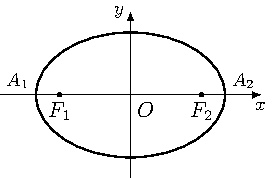
\includegraphics{ex6-1.pdf}
        \caption*{(第 \ref{exec:6-1} 题)}
      \end{minipage}
    \end{figurehere}
    \item 已知椭圆的面积公式是 $S=\uppi ab$,其中 $a$、$b$ 分别是椭圆长半轴和短半轴的长。利用这个公式,求下列椭圆的面积:
    \begin{tasks}(2)
      \task $9x^2+y^2=8$;
      \task $9x^2+25y^2=100$。
    \end{tasks}
    \item 求椭圆 $\dfrac{x^2}{16}+\dfrac{y^2}{25}=1$ 上一点 $M_1\,(2.4,4)$ 与焦点的距离。\par\smallskip
    \item 求适合下列条件的椭圆的标准方程:
    \begin{tasks}
      \task 椭圆经过两点 $P\,(-2\sqrt{2},0)$、$Q\,(0,\sqrt{5})$;
      \task 长轴是短轴的 3 倍,椭圆经过点 $P\,(3,0)$;
      \task 焦点坐标是 $(-2\sqrt{3},0)$ 和 $(2\sqrt{3},0)$,并且经过点 $P\,(\sqrt{5},-\sqrt{6})$。
      \task 离心率等于 0.8,焦距是 8。
    \end{tasks}
    \item 讨论下列椭圆的范围,并描点画出图形:
    \begin{tasks}(3)
      \task $4x^2+y^2=16$;
      \task $5x^2+9y^2=100$;
      \task $2x^2=1-y^2$。
    \end{tasks}
    \item 我国发射的科学实验人造地球卫星的运行轨道是以地球的中心为一个焦点的椭圆,近地点距地面 \qty{266}{km},远地点距地面 \qty{1826}{km}。求这颗卫星的轨道方程。
    \item 彗星“紫金山一号”是南京天文台发现的。它的运行轨道是以太阳为一个焦点的椭圆。测得轨道的近日点距太阳中心 1.486 天文单位,远日点距太阳中心 5.563 天文单位 (1 天文单位是太阳到地球的平均距离,约 \qty{1.5e8}{km}),求椭圆的方程。
    \item 已知地球运行的轨道是长半轴长 $a=\qty{1.5e8}{km}$ ,离心率 $e={0.0192}$ 的椭圆。太阳在这个椭圆的一个焦点上。求地球到太阳最大和最小的距离。
    \item 求下列椭圆的离心率:
    \begin{tasks}
      \task 从焦点看短轴两端点的视角为 \ang{60};
      \task 从短轴的一个端点看两焦点的视角为直角。
    \end{tasks}
    \item 点 $P$ 与一定点 $F\,(2,0)$ 的距离和它到一定直线 $x=8$ 的距离的比是 $1:2$。求点 $P$ 的轨迹方程,并说明轨迹是什么图形。
    \item $\triangle ABC$ 的一边的两顶点是 $B\,(0,6)$ 和 $C\,(0,-6)$,另两边的斜率的乘积是 $-\frac{4}{9}$,求顶点 $A$ 的轨迹。
    \item 点 $M$ 与椭圆 $\dfrac{x^2}{13^2}+\dfrac{y^2}{12^2}=1$ 的左焦点和右焦点的距离的比为 $2:3$。求点 $M$ 的轨迹方程,并画出图形。
    \item 已知直线和椭圆的方程如下,求它们的交点坐标:
    \begin{tasks}
      \task $3x+10y-25=0$,$\dfrac{x^2}{25}+\dfrac{y^2}{4}=1$;
      \task $3x-y+2=0$,$\dfrac{x^2}{16}+\dfrac{y^2}{4}=1$。
    \end{tasks}
    \item 求证两椭圆 $b^2x^2+a^2y^2-a^2b^2=0$,$a^2x^2+b^2y^2-a^2b^2=0$ 的交点在以原点为中心的圆周上,并求这个圆的方程。
  \end{question}
\end{Exercise}

\section{双曲线}
\subsection{双曲线及其标准方程}
我们知道,与两定点的距离的和为常数的点的轨迹是椭圆,那么与两定点的距离的差为常数的点的轨迹又是怎样的曲线: 这就是我们下面要讨论的问题。

\medskip\noindent
\begin{minipage}{0.6\linewidth}\parindent2em
平面内与两个定点 $F_1$、$F_2$ 的距离的差的绝对值是常数(小于 $|F_1F_2|$)的点的轨迹叫做\Concept{双曲线}。
这两个定点叫做双曲线的\Concept{焦点},两焦点的距离叫做\Concept{焦距}。

取过焦点 $F_1$、$F_2$ 的直线为 $x$ 轴,线段 $|F_1F_2|$ 的垂直平分线为 $y$ 轴(\cref{fig:2-19})。

设 $M\,(x,y)$ 是双曲线上的任意一点,双曲线的焦距是 $2c$($c>$),那么,$F_1$、$F_2$ 的坐标分别是 $(-c,0)$、$(c,0)$。又设点 $M$ 与 $F_1$ 和 $F_2$ 的距离的差的绝对值等于常数 $2a$。
\end{minipage}\hfill
\begin{minipage}{0.35\linewidth}\centering
  \begin{figurehere}
    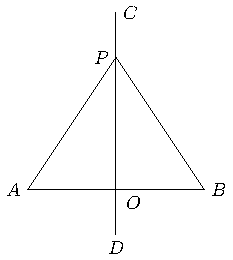
\includegraphics{2-19.pdf}
    \caption{}\label{fig:2-19}
  \end{figurehere}
\end{minipage}

\medskip
由定义可知,双曲线就是集合
\begin{gather*}
P=\bigl\{ M \bigm\vert |MF_1|-|MF_2|=\pm 2a \bigr\},\\
\because |MF_1|=\sqrt{(x+c)^2+y^2},|MF_2|=\sqrt{(x-c)^2+y^2},
\end{gather*}
得方程
\[ \sqrt{(x+c)^2+y^2}-\sqrt{(x-c)^2+y^2}=\pm 2a.\]
化简,得
\[(c^2-a^2)x^2-a^2y^2=a^2(c^2-a^2).\]

由双曲线的定义,$2c>2a$,即 $c>a$,所以 $c^2-a^2>0$,设 $c^2-a^2=b^2$($b>0$),代入上式得
\[b^2x^2-a^2y^2=a^2b^2\]
也就是
\begin{equation}
  \label{eq:hyperbola_standard_equation}
  \tcbhighmath{\frac{x^2}{a^2}-\frac{y^2}{b^2}=1}.
\end{equation}

这个方程叫做\Concept{双曲线的标准方程},它所表示的双曲线的焦点在 $x$ 轴上,焦点是 $F_1\,(-c,0)$、$F_2\,(c,0)$,这里 $c^2=a^2+b^2$。

\medskip\noindent
\begin{minipage}{0.55\linewidth}\parindent2em
如果双曲线的焦点在 $y$ 轴上(\cref{fig:2-20}),焦点是 $F_1\,(0,-c)$、$F_2\,(0,c)$,只要将\cref{eq:hyperbola_standard_equation} 的 $x$、$y$ 互换就可以得到它的方程
\[ \frac{y^2}{a^2}-\frac{x^2}{b^2}=1. \]
这个方程也是双曲线的标准方程。
\end{minipage}\hfill
\begin{minipage}{0.4\linewidth}
\begin{figurehere}
  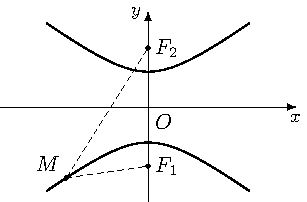
\includegraphics{2-20.pdf}
  \caption{}\label{fig:2-20}
\end{figurehere}
\end{minipage}

\medskip
\begin{example}
  已知两点 $F_1\,(-5,0)$、$F_2\,(5,0)$,求与它们的距离的差的绝对值是 6 的点的轨迹方程。
\end{example}
\begin{solution}
  按定义,所求点的轨迹是双曲线,因 $c=5$,$a=3$,所以
  \[b^2=c^2-a^2=5^2-3^2=4^2,\]
  因此所求方程是
  \[ \frac{x^2}{3^2}-\frac{y^2}{4^2}=1,\quad\text{即}\quad \frac{x^2}{9}-\frac{y^2}{16}=1.\]
\end{solution}

\begin{Practice}
  \begin{question}
    \item 求适合下列条件的双曲线的标准方程:
    \begin{tasks}
      \task $a=4$,$b=3$,焦点在 $x$ 轴上;
      \task $a=2\sqrt{5}$,经过点 $A\,(2,-5)$,焦点在 $y$ 轴上。
    \end{tasks}
    \item 证明:椭圆 $\dfrac{x^2}{25}+\dfrac{y^2}{9}=1$ 与双曲线 $x^2-15y^2=15$ 的焦点相同。
  \end{question}
\end{Practice}

\subsection{双曲线的几何性质}
我们根据双曲线的标准方程
\[ \frac{x^2}{a^2}-\frac{y^2}{b^2}=1,\]
来研究它的几何性质。
\subsubsection{范围}
由标准方程可知,双曲线上点的坐标 $(x,y)$,对于任何实数 $x$,$y$ 都适合不等式 $\dfrac{x^2}{a^2} \geqslant 1$,即 $x^2 \geqslant a^2$。

$\therefore \quad x \geqslant a$ 或 $x \leqslant -a$。

这说明双曲线在两条直线 $x=a$,$x=-a$ 的外侧。

\subsubsection{对称性}
双曲线关于每个坐标轴和原点都是对称的。
这时,坐标轴是双曲线的对称轴,原点是双曲线的对称中心。
双曲线的对称中心叫做双曲线的\Concept{中心}。

\subsubsection{顶点}
\noindent
\begin{minipage}{0.6\linewidth}\parindent2em
在标准方程中,令 $y=0$,得 $x=\pm a$,因此双曲线和 $x$ 轴有两个交点 $A_1\,(-a,0)$、$A_2\,(a,0)$。
因为 $x$ 轴是双曲线的对称轴,所以双曲线和它的对称轴有两个交点,它们叫做双曲线的\Concept{顶点}。

令 $x=0$,得 $y^2=-b^2$,这个方程没有实数根,说明双曲线和 $y$ 轴没有交点,但我们也把 $B_1\,(0,-b)$、$B_2\,(0,b)$ 画在 $y$ 轴上(\cref{fig:2-21})。
\end{minipage}\hfill
\begin{minipage}{0.35\linewidth}\centering
\begin{figurehere}
  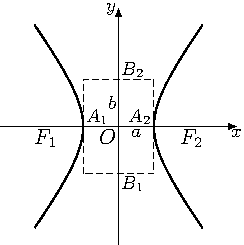
\includegraphics{2-21.pdf}
  \caption{}\label{fig:2-21}
\end{figurehere}
\end{minipage}

\medskip
线段 $A_1A_2$ 叫做双曲线的\Concept{实轴},它的长等于 $2a$,$a$ 叫做双曲线的实半轴长。
线段 $B_1B_2$ 叫做双曲线的\Concept{虚轴},它的长等于 $2b$,$b$ 叫做双曲线的虚半轴长。

\subsubsection{渐近线}
\noindent
\begin{minipage}{0.6\linewidth}\parindent2em\linespread{1.6}\selectfont
经过 $A_2$、$A_1$ 作 $y$ 轴的平行线 $x=\pm a$,经过 $B_2$、$B_1$ 作 $x$ 轴的平行线 $y=\pm b$,四条直线围成一个矩形(\cref{fig:2-22})。矩形的两条对角线所在直线的方程是 $y=\pm\dfrac{b}{a}x$,从\cref{fig:2-22} 可以看出,双曲线 $\dfrac{x^2}{a^2}-\dfrac{y^2}{b^2}=1$ 的各支向外延伸时,与这两条直线逐渐接近。
\end{minipage}\hfill
\begin{minipage}{0.35\linewidth}\centering
\begin{figurehere}
  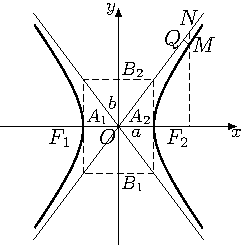
\includegraphics{2-22.pdf}
  \caption{}\label{fig:2-22}
\end{figurehere}
\end{minipage}

下面,我们来证明这个事实。

双曲线在第一象限内的一部分的方程可写为
\[y=\frac{b}{a}\sqrt{x^2-a^2}\quad(x>a),\]
设 $M\,(x,y)$ 是它上面的点,$N\,(x,Y)$ 是直线 $y=\dfrac{b}{a}x$ 上与 $M$ 有相同横坐标的点,则 $Y=\dfrac{b}{a}x$。

设 $|MQ|$ 是点 $M$ 到直线 $y=\dfrac{b}{a}x$ 的距离,则 $|MQ|<|MN$。当 $x$ 逐渐增大时,$|MN|$ 逐渐减小,$x$ 无限增大,$|MN|$ 接近于零,$|MQ|$ 也接近于零,就是说,双曲线在第一象限的部分从射线 $ON$ 的下方逐渐接近于射线 $ON$。

在其他象限内也可以证明类似的情况。
我们把两条直线 $y=\pm\dfrac{b}{a}x$ 叫做双曲线的\Concept{渐近线}。
在方程 $\dfrac{x^2}{a^2}-\dfrac{y^2}{b^2}=1$ 中,如果 $a=b$,那么双曲线方程为 $x^2-y^2=a^2$,它的实轴和虚轴的长都等于 $2a$。
这时,四条直线 $x=\pm a$,$y=\pm a$ 围成正方形,渐近线方程成为 $x=\pm y$,它们互相垂直,并且平分双曲线实轴和虚轴所成的角。
实轴和虚轴等长的双曲线叫做\Concept{等轴双曲线}。

\subsubsection{离心率}
双曲线的焦距与实轴的比 $e=\dfrac{c}{a}$,叫做双曲线的\Concept{离心率}。因为 $c> a$,所以双曲线的离心率 $e>1$。

由等式 $c^2-a^2=b^2$ 可得
\[\frac{b}{a}=\frac{\sqrt{c^2-a^2}}{a}=\sqrt{\frac{c^2}{a^2}-1}=\sqrt{e^2-1} .\]
因此 $e$ 越大,$\dfrac{b}{a}$ 也越大,即渐近线 $y=\pm\dfrac{b}{a}x$ 的斜率的绝对值越大,这时双曲线的形状就从扁狭逐渐变得开阔。
由此可知,双曲线的离心率越大,它的开口就越开阔。

\begin{example}
  求双曲线 $9y^2-16x^2=144$ 的实半轴长和虚半轴长、焦点坐标、离心率、渐近线方程。
\end{example}
\begin{solution}
  把方程化为标准方程
  \[ \frac{y^2}{4^2}-\frac{x^2}{3^2}=1. \]
  
  由此可知,实半轴长 $a=4$,虚半轴长 $b=3$。
  \[c = \sqrt{{a}^{2} + {b}^{2}} = \sqrt{{4}^{2} + {3}^{2}} = 5.\]
  
  焦点的坐标是 $(0,-5)$,$(0,5)$。

  离心率 $e=\dfrac{c}{a}=\dfrac{5}{4}$。

  渐近线方程为
  \[x=\pm\frac{3}{4}y,\quad\text{即}\quad y=\pm\frac{4}{3}x.\]
\end{solution}
\begin{example}
  双曲线型自然通风塔的外形,是双曲线的一部分绕其虚轴旋转所成的曲面(\cref{fig:2-23}),它的最小半径为 \qty{12}{m},上口半径为 \qty{13}{m},下口半径为 \qty{25}{m},高 \qty{55}{m}。在所给的坐标系中求此双曲线的方程。
\end{example}
\begin{figure}
  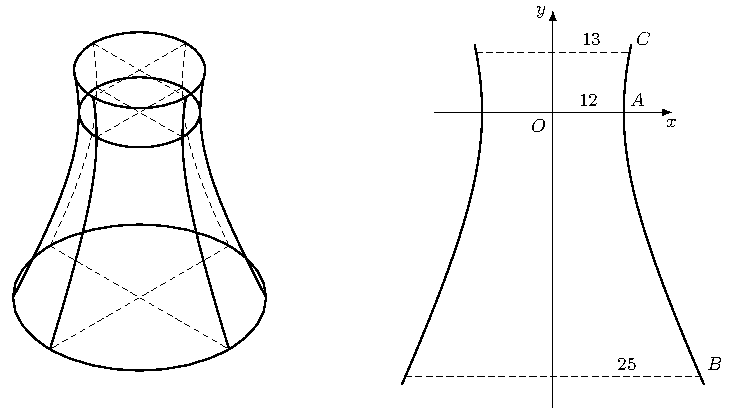
\includegraphics{2-23.pdf}
  \caption{}\label{fig:2-23}
\end{figure}
\begin{solution}
  在\cref{fig:2-23} 的坐标系中,双曲线有标准方程
  \[\frac{x^2}{a^2}-\frac{y^2}{b^2}=1\]
  
  点 $A$ 旋转所成的圆半径最小,$a=12$。下面求 $b$。

设 $B$ 是双曲线上位于通风塔下口的一点,它的坐标为 $(25,y_1)$;$C$ 是双曲线上位于通风塔上口的一点,它的坐标为 $(13,y_2)$。因为 $B$、$C$ 在双曲线上,所以
\begin{align*}
  \frac{25^2}{12^2} -\frac{y_1^2}{b^2}&= 1,\\
  \frac{13^2}{12^2} -\frac{y_2^2}{b^2}&= 1.
\end{align*}
解得
\begin{align*}
  y_1&=-\frac{b}{12}\sqrt{25^2-12^2}=-\frac{b}{12}\sqrt{481},\\
  y_2&=\frac{b}{12}\sqrt{13^2-12^2}=\frac{5}{12}b.
\end{align*}
因为塔高 \qty{55}{m},所以 $y_2-y_1=55$。即
\[\frac{5}{12}+\frac{b\sqrt{481}}{12}=55.\]
解得
\[b \approx \qty{24.5}{m}.\]
所以双曲线方程(近似)为
\[\frac{x^2}{12^2}-\frac{y^2}{24.5^2}=1.\]
\end{solution}
\begin{example}
  以已知双曲线的虚轴为实轴,实轴为虚轴的双曲线叫做原双曲线的\Concept{共轭双曲线}。求证:
  \begin{enumerate}
    \item 双曲线和它的共轭双曲线有共同的渐近线;
    \item 双曲线和它的共轭双曲线的四个焦点在同一个圆上。
  \end{enumerate}
\end{example}
\begin{proof}
  \begin{enumerate}
    \item 设已知双曲线的方程是
    \[\frac{x^2}{a^2}-\frac{y^2}{b^2}=1\]
  \end{enumerate}
  \begin{minipage}{0.5\linewidth}\parindent2em
    \noindent 根据定义,它的共轭双曲线的方程是
    \[\frac{y^2}{b^2}-\frac{x^2}{a^2}=1.\]

    已知双曲线的渐近线方程是
    \[y=\pm\frac{b}{a}x,\]
    它的共轭双曲线的渐近线方程是
    \[x=\pm\frac{a}{b}y,\quad\text{即}\quad y=\pm\frac{b}{a}x.\]
  \end{minipage}\hfill
  \begin{minipage}{0.45\linewidth}\centering
    \begin{figurehere}
      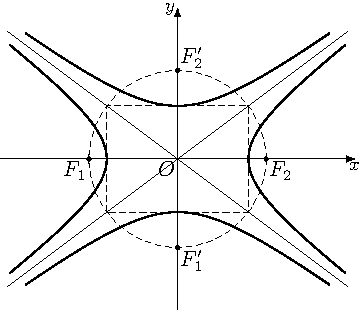
\includegraphics{2-24.pdf}
      \caption{}\label{fig:2-24}
    \end{figurehere}
  \end{minipage}\par\medskip 
  所以双曲线和它的共轭双曲线有共同的渐近线。
  \begin{enumerate}[resume]
    \item 设已知双曲线的焦点为 $F_1\,(-c,0)$、$F_2\,(c,0)$,它的共轭双曲线的焦点为 $F'_1\,(0,-c')$、$F'_2\,(0,c')$。
    
    $\because \quad c=\sqrt{a^2+b^2}$,$c'=\sqrt{b^2+a^2}$,

    $\therefore \quad c=c'$。
    
    所以四个焦点 $F_1$、$F_2$、$F'_1$、$F'_2$ 在同一个圆 $x^2+y^2=a^2+b^2$ 上(\cref{fig:2-24})。
  \end{enumerate}
\end{proof}
\begin{example}
  点 $M\,(x,y)$ 到定点 $F\,(c,0)$ 的距离和它到定直线 $l:x=\dfrac{a^2}{c}$ 的距离的比是常数 $\dfrac{c}{a}$($c>a>0$)。求点 $M$ 的轨迹\cref{fig:2-25})。
\end{example}

\noindent
\begin{minipage}{0.55\linewidth}\parindent2em
\begin{solution}
  设 $d$ 是点 $M$ 到直线 $l$ 的距离。根据题意,所求轨迹,就是集合
  \[P=\left\{ M \middle\vert \frac{|MF|}{d}=\frac{c}{a} \right\},\]
  由此得
  \[ \frac{\sqrt{(x-c)^2+u^2}}{\left|x-\dfrac{a^2}{c}\right|}=\frac{c}{a}.\]
\end{solution}
\end{minipage}\hfill
\begin{minipage}{0.4\linewidth}\centering
  \begin{figurehere}
    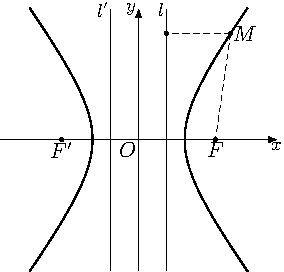
\includegraphics{2-25.pdf}
    \caption{}\label{fig:2-25}
  \end{figurehere}
\end{minipage}

\medskip\noindent
化简,得
\[(c^2-a^2)x^2-a^2y^2=a^2(c^2-a^2).\]
设 $c^2-a^2=b^2$,就可化为
\[\frac{x^2}{a^2}-\frac{y^2}{b^2}=1,\]
这是双曲线的标准方程。

因此,点 $M$ 到一个定点的距离和它到一条定直线的距离的比是常数 $e=\dfrac{c}{a}$($e>1$)时,这个点的轨迹是双曲线。
定点是焦点,定直线叫做双曲线的\Concept{准线},常数 $e$ 是双曲线的离心率。

对于双曲线 $\dfrac{x^2}{a^2}-\dfrac{y^2}{b^2}=1$,相应于焦点 $F\,(c,0)$ 的准线方程是 $x=\dfrac{a^2}{c}$。
根据双曲线的对称性,相应于焦点 $F'\,(-c,0)$ 的准线方程是 $x=-\dfrac{a^2}{c}$。
所以双曲线有两条准线。

\begin{Practice}
  \begin{question}
    \item 求下列双曲线的实轴和虚轴的长、顶点和焦点坐标、离心率、渐近线方程和准线方程:
    \begin{tasks}(2)
      \task $x^2-8y^2=32$;
      \task $9x^2-y^2=81$;
      \task $x^2-y^2=-4$;
      \task $\dfrac{x^2}{49}-\frac{y^2}{25}=-1$。
    \end{tasks}
    \item 求适合下列条件的双曲线的标准方程:
    \begin{tasks}
      \task 顶点在 $x$ 轴上,两顶点的距离是 8,$e=\dfrac{5}{4}$;
      \task 焦点在 $y$ 轴上,焦距是 16,$e= \dfrac{4}{3}$;
      \task 一条渐近线的方程是 $3x-2y=0$,实轴长为 8。
    \end{tasks}
    \item 等轴双曲线的一个焦点是 $F_1\,(-6,0)$,求它的标准方程和渐近线方程。
  \end{question}
\end{Practice}
\begin{Exercise}
  \begin{question}
    \item 根据下列条件,求双曲线的标准方程:
    \begin{tasks}
      \task 焦点的坐标是 $(-6,0)$、$(6,0)$,并且经过点 $A\,(-5,2)$;
      \task 经过点 $P\,(-3,,2\sqrt{7})$ 和 $Q\,(-6\sqrt{2},-7)$,焦点在 $y$ 轴上。
    \end{tasks}
    \item 参考椭圆的画法,根据双曲线的定义,研究一下怎样用直尺和圆规作点画出双曲线。
    \item 已知双曲线的方程是:
    \begin{tasks}(2)
      \task $16x^2-9y^2=144$;
      \task $16x^2-9y^2=-144$,
    \end{tasks}
    求它的焦点坐标、离心率、渐近线方程。
    \item 求双曲线的标准方程:
    \begin{tasks}
      \task 实轴的长是 10,虚轴的长是 8,焦点在 $x$ 轴上;
      \task 焦距是 10,虚轴的长是 8,焦点在 $y$ 轴上;
      \task 离心率 $e=\sqrt{2}$,经过点 $M\,(-5,3)$;
      \task 两条渐近线的方程是 $y=\pm\dfrac{2}{3}x$,经过点 $M\,(\dfrac{9}{2},-1)$。
    \end{tasks}
    \item 求与椭圆 $\dfrac{x^2}{49}+\dfrac{y^2}{24}=1$ 有公共焦点,且离心率 $e= \dfrac{5}{4}$ 的双曲线方程。
    \item 求以椭圆 $\dfrac{x^2}{8}+\dfrac{y^2}{5}=1$ 的焦点为顶点,而以椭圆的顶点为焦点的双曲线方程。
    \item 求与双曲线 $\dfrac{x^2}{9}-\dfrac{y^2}{16}=1$ 有共同的渐近线,且经过点 $A\,(-3,2\sqrt{3})$ 的双曲线方程。
    \item 求经过点 $A\,(3,-1)$,并且对称轴都在坐标轴上的等轴双曲线的方程。
    \item 证明:等轴双曲线的离心率是 $\sqrt{2}$。
    \item 在相距 \qty{1400}{m} 的 $A$、$B$ 两哨所,听到炮弹爆炸声的时间相差 \qty{3}{s},已知声速是 \qty{340}{m/s}。炮弹爆炸点在怎样的曲线上?
    \item 通过双曲线 $\dfrac{x^2}{144}-\dfrac{y^2}{25}=1$ 的一个焦点,作 $x$ 轴的垂线,求垂线与双曲线的交点与两焦点的距离。
    \item 证明从双曲线的一个焦点到一条渐近线的距离等于虚半轴长。
    \item 求下列直线和双曲线的交点坐标:
    \begin{tasks}
      \task $2x-y-10=0$,$\dfrac{x^2}{20}-\dfrac{y^2}{5}=1$;
      \task $4x-3y-16=0$,$\dfrac{x^2}{25}-\dfrac{y^2}{16}=1$。
    \end{tasks}
    \item 证明椭圆 $\dfrac{x^2}{20}+\dfrac{y^2}{5}=1$ 与双曲线 $\dfrac{x^2}{12} - \dfrac{y^2}{3}=1$ 的交点是一矩形的顶点。
    \item 求与定点 $A\,(5,0)$ 及定直线 $l:x=\dfrac{16}{5}$ 的距离比是 $5:4$ 的点的轨迹方程。
    \item $\triangle ABC$ 一边的两个端点是 $B\,(0,6)$ 和 $C\,(0,-6)$,另两边斜率的积是 $\dfrac{4}{9}$,求顶点 $A$ 的轨迹。
    \item 判定当 
    \begin{tasks}(2)
      \task $k<4$;
      \task $4<k<9$
    \end{tasks}
    时,方程 $\dfrac{x^2}{9-k}+\dfrac{y^2}{4-k}=1$ 分别表示什么曲线。\par\medskip
    \item 当 $\alpha$ 从 \ang{0} 到 \ang{180} 变化时,曲线 $x^2+y^2\cos\alpha=1$ 怎样变化?
  \end{question}
\end{Exercise}

\section{抛物线}
\subsection{抛物线及其标准方程}
\medskip\noindent
\begin{minipage}{0.7\linewidth}\parindent2em
我们知道,与一个定点的距离和一条定直线的距离的比是常数 $e$ 的点的轨迹,当 $e<1$ 时,是椭圆,当 $e>1$ 时,是双曲线。
那么,当 $e=1$ 时,它又是什么曲线?

平面内与一个定点 $F$ 和一条定直线 $l$ 的距离相等的点的轨迹叫做抛物线。
点 $F$ 叫做抛物线的\Concept{焦点}。
直线 $l$ 叫做抛物线的\Concept{准线}。

取经过焦点 $F$ 且垂直于准线 $l$ 的直线为 $x$ 轴,$x$ 轴与 $l$ 相交于点 $K$,以线段 $KF$ 的垂直平分线为 $y$ 轴(\cref{fig:2-26})。
设 $|KF|=p$,那么,焦点 $F$ 的坐标为 $\left(\dfrac{p}{2},0\right)$,准线 $l$ 的方程为 $x=-\dfrac{p}{2}$。
\end{minipage}\hfill
\begin{minipage}{0.25\linewidth}
\begin{figurehere}
  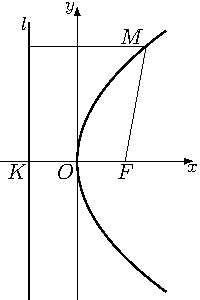
\includegraphics{2-26.pdf}
  \caption{}\label{fig:2-26}
\end{figurehere}
\end{minipage}

\medskip
设抛物线上的点 $M\,(x,y)$ 到 $l$ 的距离为 $d$。抛物线也就是集合
\[P=\bigl\{ M \bigm\vert |MF|=d \bigr\}.\]
\begin{align*}
  \because \quad |MF|&= \sqrt{\left(x-\frac{P}{2}\right)^2+y^2},\\
  d&= \left|x+\frac{P}{2}\right|,\\
  \therefore \quad \sqrt{\left(x-\frac{P}{2}\right)^2+y^2}&= \left|x+\frac{P}{2}\right|.
\end{align*}
将上式两边平方,并化简得
\begin{equation}
  \label{eq:parabola_standard_equation}
  \tcbhighmath{y^2=2px\quad(p>0)}.
\end{equation}

\cref{eq:parabola_standard_equation}叫做\Concept{抛物线的标准方程}。
它表示的抛物线的焦点在 $x$ 轴的正半轴上,坐标是 $\left(\dfrac{p}{2},0\right)$,准线方程是 $x=-\dfrac{p}{2}$。

\medskip
一条抛物线,由于它在坐标平面上的位置不同,方程也不同。
所以抛物线的标准方程还有其他几种形式:$y^2=-2px$、$x^2=2py$、$x^2=-2py$。它们的焦点坐标,准线方程以及图形列表如\cref{tab:2-1}:
\begin{table}
  \caption{几种抛物线的焦点坐标,准线方程以及图形}\label{tab:2-1}
  \begin{tblr}{colspec={*4{X[c]}},hline{2}={0.8pt}}
    方程 & 焦点 & 准线 & 图形 \\
    $y^2=2px\,\,(p>0)$  & $F\,\left(\dfrac{p}{2},0\right)$    & $x=-\dfrac{p}{2}$ &\begin{minipage}{3cm}\centering 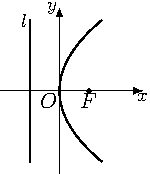
\includegraphics{parabola1.pdf}\end{minipage}\\
    $y^2=-2px\,\,(p>0)$ & $F\,\left(-\dfrac{p}{2},0\right)$   & $x=\dfrac{p}{2}$  &\begin{minipage}{3cm}\centering 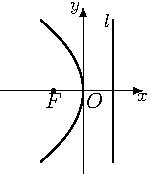
\includegraphics{parabola2.pdf}\end{minipage} \\
    $x^2=2py\,\,(p>0)$  & $F\,\left(0,\dfrac{p}{2},0\right)$  & $y=-\dfrac{p}{2}$ &\begin{minipage}{3cm}\centering 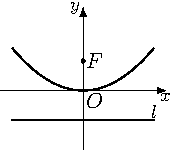
\includegraphics{parabola3.pdf}\end{minipage} \\
    $x^2=-2py\,\,(p>0)$ & $F\,\left(0,-\dfrac{p}{2},0\right)$ & $y=\dfrac{p}{2}$  &\begin{minipage}{3cm}\centering 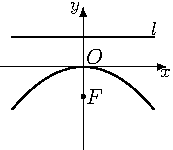
\includegraphics{parabola4.pdf}\end{minipage} \\
  \end{tblr}
\end{table}

\begin{example}\mbox{}\par
  \begin{enumerate}
    \item 已知抛物线的标准方程是 $y^2=6x$,求它的焦点坐标和准线方程;
    \item 已知抛物线的焦点坐标是 $F\,(0,-2)$,求它的标准方程。
  \end{enumerate}
\end{example}
\begin{solution}
  \begin{enumerate}
    \item 因为 $p=3$,所以焦点坐标是 $\left(\dfrac{3}{2},0\right)$,准线方程是 $x=-\dfrac{3}{2}$。
    \item 因为焦点在 $y$ 轴的负半轴上,并且 $\dfrac{p}{2}=2$,$p=4$,所以它的标准方程是
    \[ x^2=-8y.\]
  \end{enumerate}
\end{solution}

\begin{example}
  在工程中,画拱宽为 $2a$,拱高为 $h$ 的抛物线,常用下面画法。
  证明画法的正确性。
  \begin{enumerate}
    \item 作矩形 $ABCD$ ,使 $AB=2a$,$DA=h$(\cref{fig:2-27})。
    \item 取 $CD$ 的中点 $O$,把线段 $DA$、$OD$ 各 $n$ 等分。设 $OD$ 上的分点顺次为 $A_1$、$A_2$、$\cdots$,$DA$ 上的分点顺次为 $B_1$、$B_2$、$\cdots$。
    \item 过 $O$、$A_1$、$A_2$、$\cdots$ 作直线 $OH$、$A_1A'_1$、$A_2A'_2$、$\cdots$ 平行于 $DA$,交 $AB$ 于 $H$、$A'_1$、$A'_2$、$\cdots$。连结 $OB_1$、$OB_2$、$\cdots$ 分别交 $A_1A'_1$、$A_2A'_2$、$\cdots$ 于 $P_1$、$P_2$、$\cdots$。把 $O$、$P_1$、$P_2$、$\cdots$、$A$ 各点连成光滑曲线,就得到拱形的一半。
    \item 用同样方法画出另一半。
  \end{enumerate}
\end{example}
\begin{figure}
  \begin{minipage}[b]{0.43\linewidth}\centering
    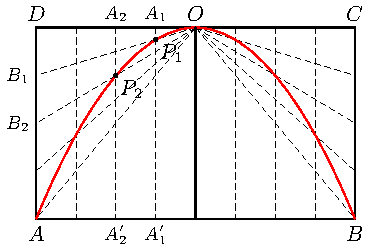
\includegraphics{2-27.pdf}
    \caption{}\label{fig:2-27}
  \end{minipage}
  \begin{minipage}[b]{0.52\linewidth}\centering
    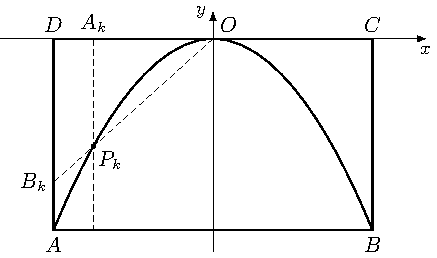
\includegraphics{2-28.pdf}
    \caption{}\label{fig:2-28}
  \end{minipage}
\end{figure}
\begin{proof}
  以 $O$ 为原点,直线 $DC$ 为 $x$ 轴建立直角坐标系(\cref{fig:2-28})。

  设 $P_k$ 是上面所作的任意一点,由画法可知,$P_k$ 是直线 $A_kA'_k$ 与 $OB_k$ 的交点。$A_kA'_k$ 的方程是 $x=-\dfrac{k}{n}a$,$OB_k$ 的方程是 $y=\dfrac{kh}{na}x$,由方程组
  \[ \begin{cases} x=-\dfrac{k}{n}a, \\[10pt] y=\dfrac{kh}{na}x\end{cases}\]
  消去 $\dfrac{k}{n}$,得方程
  \[ x^2=-\frac{a^2}{h}y.\]
  这就是说,点 $P_k$ 的坐标 $x$、$y$ 满足抛物线方程,所以所画的拱形是一段抛物线。
\end{proof}

\begin{Practice}
  \begin{question}
    \item 根据抛物线的定义,仿照椭圆和双曲线的画法,利用直尺和圆规作点画出焦点到准线的距离等于 $p$ 的抛物线。
    \item 根据下列所给的条件,写出抛物线的标准方程:
    \begin{tasks}(2)
      \task 焦点是 $F\,(3,0)$;
      \task 准线方程是 $x=-\dfrac{1}{4}$;
      \task 焦点到准线的距离是 2。
    \end{tasks}
    \item 求下列抛物线的焦点坐标和准线方程:
    \begin{tasks}(2)
      \task $y^2=20x$;
      \task $x^2=\dfrac{1}{2}y$;
      \task $2y^2+5x= 0$;
      \task $x^2+8y= 0$。
    \end{tasks}
  \end{question}
\end{Practice}
\subsection{抛物线的几何性质}
我们根据抛物线的标准方程
\begin{equation}
  \label{eq:parabolar_standard_equation_2}
  y^2=2px\quad(p>0),
\end{equation}
来研究它的几何性质。

\subsubsection{范围}
因为 $p>0$,由\cref{eq:parabolar_standard_equation_2} 可知,对于抛物线 \eqref{eq:parabolar_standard_equation_2} 的点 $M\,(x,y)$,$x\geqslant 0$,所以这条抛物线在 $y$ 轴的右侧,当 $x$ 的值增大时,$|y|$ 也增大,这说明抛物线向右上方和右下方无限延伸。

\subsubsection{对称性}
以 $-y$ 代 $y$,\cref{eq:parabolar_standard_equation_2} 不变,所以这个抛物线关于 $x$ 轴对称,我们把抛物线的对称轴叫做抛物线的\Concept{轴}。

\subsubsection{顶点}
抛物线和它的轴的交点叫做抛物线的\Concept{顶点}。在\cref{eq:parabolar_standard_equation_2} 中,当 $y=0$ 时,$x=0$,因此抛物线 \eqref{eq:parabolar_standard_equation_2} 的顶点就是坐标原点。

\subsubsection{离心率}
抛物线上的点 $M$ 与焦点和准线的距离的比,叫做抛物线的\Concept{离心率},用 $e$ 表示。按抛物线的定义,$e=1$ 。

\begin{example}
  已知抛物线关于 $x$ 轴对称,它的顶点在坐标原点,且经过点 $M\,(2,- 2\sqrt{2})$。求它的标准方程,并用描点法画出图形。
\end{example}
\noindent
\begin{minipage}{0.7\linewidth}\parindent2em
\begin{solution}
  因为抛物线关于 $x$ 轴对称,它的顶点在坐标原点,并且经过点 $M\,(2,- 2\sqrt{2})$,所以可设它的标准方程为
  \[ y^2=2px.\]
  因为点 $M$ 在抛物线上,所以
  \[ (-2\sqrt{2})^2=2p\cdot 2,\]
  即
  \[ p=2.\]
  因此所求方程是
  \[ y^2=4x.\]
\end{solution}
\end{minipage}\hfill
\begin{minipage}{0.25\linewidth}\centering
\begin{figurehere}
  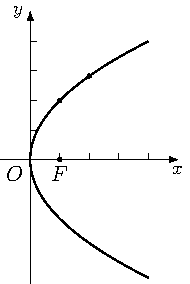
\includegraphics{2-29.pdf}
  \caption{}\label{fig:2-29}
\end{figurehere}
\end{minipage}

\medskip
将已知方程变形为 $y=\pm2\sqrt{x}$,根据 $y=2\sqrt{x}$ 计算抛物线在第一象限内的几个点的坐标,得
  \begin{tablehere}
    \begin{tblr}{colspec={*7{X[c]}},vline{2}={0.8pt}}
      $x$ & 0&1 & 2& 3& 4& $\cdots$ \\
      $y$ & 0& 2& 2.8& 3.5& 4& $\cdots$ \\
    \end{tblr}
  \end{tablehere}
  描点画出抛物线在第一象限内的一部分,再利用对称性,就可以画出抛物线的另一部分 (\cref{fig:2-29})。

\begin{example}
  探照灯 反射镜的纵断面是抛物线的一部分。灯口直径是 \qty{60}{cm},灯深 \qty{40}{cm}。求抛物线的标准方程和焦点的位置。
\end{example}
\noindent
\begin{minipage}{0.65\linewidth}\parindent2em
\begin{solution}
  在纵断面内,以反射镜的顶点(即抛物线的顶点)为坐标原点,过顶点垂直于灯口直径的直线为 $x$ 轴,建立直角坐标系(\cref{fig:2-30})。

设抛物线的标准方程是 $y^2=2px$。因为点 $A$ 的坐标是 $(40,30)$,代入方程,得
\[ 30^2=2p\times 40,\]
即
\[ p=\frac{45}{4}.\]
\end{solution}
\end{minipage}\hfill
\begin{minipage}{0.3\linewidth}\centering
  \begin{figurehere}
  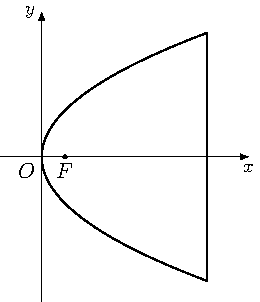
\includegraphics{2-30.pdf}
  \caption{}\label{fig:2-30}
  \end{figurehere}
\end{minipage}

\medskip
所以抛物线的方程是 $y^2=\dfrac{45}{2}x$,焦点坐标是 $\left(\dfrac{45}{8},0\right)$。

\begin{Practice}
  \begin{question}
    \item 求适合下列条件的抛物线方程:
    \begin{tasks}
      \task 顶点在原点,关于 $x$ 轴对称,并且经过点 $M\,(5,-4)$;
      \task 顶点在原点,焦点是 $F\,(0,5)$;
      \task 顶点在原点,准线是 $x=4$;
      \task 焦点是 $F\,(0,-8)$,准线是 $y=8$。
    \end{tasks}
    \item 一条隧道的顶部是抛物拱形,拱高是 \qty{1.1}{m},跨度是 \qty{2.2}{m}。求拱形的抛物线方程。
    \item 证明:与抛物线的轴平行的直线和抛物线只有一个交点。
  \end{question}
\end{Practice}

\begin{Exercise}
  \begin{question}
    \item 抛物线 $y^2=2px$($p>0$)上一点 $M$ 到焦点的距离是 $a\;\left(a> \dfrac{p}{2}\right)$,点 $M$ 到准线的距离是多少? 点 $M$ 的横坐标是多少?
    \item 取经过焦点 $F$ 且垂直于准线 $l$ 的直线为 $y$ 轴,推导抛物线的标准方程。
    \item 求下列抛物线的焦点坐标和准线方程:
    \begin{tasks}(2)
      \task $x^2=2y$;
      \task $4x^2+3y=0$;
      \task $2y^2+5x=0$;
      \task $y^2-6x=0$。
    \end{tasks}
    \item 根据下列条件,求抛物线的方程,并描点画出图形:
    \begin{tasks}
      \task 顶点在原点,对称轴是 $x$ 轴,并且顶点与焦点的距离等于 6;
      \task 顶点在原点,对称轴是 $y$ 轴,并经过点 $P\,(-6,-3)$。
    \end{tasks}
    \item 经过抛物线 $y^2=2px$ 的焦点 $F$,作一条直线垂直于它的对称轴,和抛物线相交于 $P_1$、$P_2$ 两点,线段 $P_1P_2$ 叫做抛物线的通径。求通径 $P_1P_2$ 的长。
    \item 在抛物线 $y^2=12x$ 上,求和焦点的距离等于 9 的点的坐标。
    \item 有一正三角形的两个顶点在抛物线 $y^2=2px$ 上,另一顶点在原点。求这个三角形的边长。
    \item 过抛物线 $y^2=2px$ 的焦点的一条直线和这抛物线相交,两个交点的纵坐标为 $y_1$、$y_2$。求证:$y_1y_2=-p^2$。
    \item \label{exec:8-9} 吊车梁的鱼腹部分 $AOB$ 是一段抛物线,宽为 \qty{7}{m},高为 \qty{0.7}{m},求这条抛物线的方程。
    \begin{figurehere}
      \begin{minipage}[b]{0.48\linewidth}\centering
        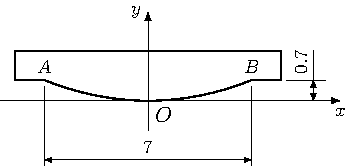
\includegraphics{ex8-9.pdf}
        \caption*{(第 \ref{exec:8-9} 题)}
      \end{minipage}
      \begin{minipage}[b]{0.48\linewidth}\centering
        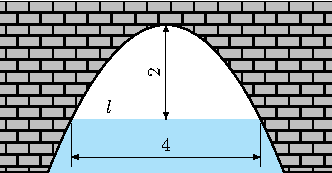
\includegraphics{ex8-10.pdf}
        \caption*{(第 \ref{exec:8-10} 题)}
      \end{minipage}
    \end{figurehere}
    \item \label{exec:8-10}图中是抛物线形拱桥,当水面在 $l$ 时,拱顶离水面 \qty{2}{m},水面宽 \qty{4}{m}。水下降 \qty{1}{m} 后,水面宽多少?
    \item 抛物线的顶点是双曲线 $16x^2-9y^2=144$ 的中心,而焦点是双曲线的左顶点。求抛物线的方程。
    \item 已知两抛物线的顶点在原点,而焦点分别在点 $F_1\,(2,0)$ 和点 $F_2\,(0,2)$。求它们的交点。
    \item 过抛物线焦点的一条直线与它交于两点 $P$、$Q_8$。通过点 $P$ 和抛物线顶点的直线交准线于点 $M$,求证: 直线 $MQ$ 平行于抛物线的对称轴。
    \item 点 $M$ 与点 $F\,(4,0)$ 的距离比它到直线 $x+5=0$ 的距离小 1,求点 $M$ 的轨迹方程,并且画出图形。
  \end{question}
\end{Exercise}

\subsection{圆锥曲线的切线和法线}
圆、椭圆、双曲线和抛物线统称\Concept{圆锥曲线}。
圆锥曲线的切线和法线的性质,在光学上有很多应用。
为了研究它们的性质,我们来研究什么叫圆锥曲线的切线和法线,并求出它们的方程。

设直线 $l'$ 与圆锥曲线相交于 $P$、$Q$ 两点(\cref{fig:2-31})。
将直线 $l'$ 绕点 $P$ 旋转,使点 $Q$ 逐渐靠近点 $P$,当 $l'$ 转到直线 $l$ 的位置时,点 $Q$ 与点 $P$ 重合,这时,直线 $l$ 叫做圆锥曲线在点 $P$ 的\Concept{切线},$P$ 叫\Concept{切点}。
经过点 $P$ 与切线垂直的直线叫做圆锥曲线在点 $P$ 的\Concept{法线}。
\begin{figure}
  \begin{minipage}[b]{0.48\linewidth}\centering
    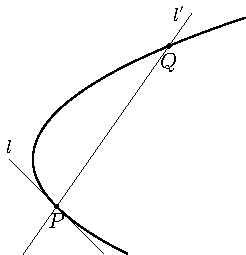
\includegraphics{2-31.pdf}
    \caption{}\label{fig:2-31}
  \end{minipage}
  \begin{minipage}[b]{0.48\linewidth}\centering
    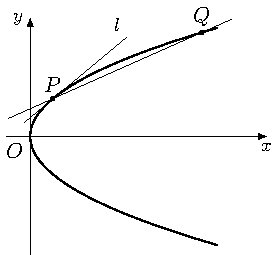
\includegraphics{2-32.pdf}
    \caption{}\label{fig:2-32}
  \end{minipage}
\end{figure}

根据圆锥曲线切线的定义,先求抛物线的切线方程。

设 $P\,(x_0,y_0)$($x_0\neq 0$)是抛物线 $y^2=2px$ 上一点,经过点 $P$ 的直线与抛物线交于另一点 $Q$(\cref{fig:2-32}),直线 $PQ$ 的方程可写成
\[ y-y_0=k(x-x_0)\quad(k \neq 0).\]

下面,我们来确定当这条直线成为切线时 $k$ 的值。

因为直线 $PQ$ 与抛物线的交点 $P$、$Q$ 的坐标是方程组
\begin{numcases}{}
  \label{eq:parabola_equation} y^2=2px,\\
  \label{eq:parabola_tangent}y-y_0=k(x-x_0)
\end{numcases}
的解,由切线定义可知,当直线 $PQ$ 与抛物线相切时,点 $Q$ 与点 $P$ 重合,因此,这时方程组应有两个相同的实数解。
根据这个条件,可以确定 $k$ 的值。

由 \eqref{eq:parabola_equation},得
\begin{equation} 
  \label{eq:parabola_equation_other}
  x=\frac{y^2}{2p},
\end{equation}
因为点 $P\,(x_0,y_0)$ 在抛物线上,所以
\begin{equation} 
  \label{eq:point_on_parabola}
  x_0=\frac{y_0^2}{2p}.
\end{equation}

将\cref{eq:parabola_equation_other,eq:point_on_parabola}代入\cref{eq:parabola_tangent},得
\[y-y_0=k\left(\frac{y^2}{2p}-\frac{y_0^2}{2p}\right),\]
即
\[ ky^2-2py+(2py_0-ky_0^2)=0.\]

这是一个关于 $y$ 的一元二次方程,它有相等的实数解的充要条件是判别式等于零,即
\begin{gather*}
  4p^2-4k(2py_0-ky_0^2)=0,\\
  (p-ky_0)^2=0.
\end{gather*}
由此得
\[k=\frac{p}{y_0}.\]
于是得到切线的方程
\[y-y_0=\frac{p}{y_0}(x-x_0).\]
因为 $y_0^2=2px_0$,上式可化简为
\begin{equation}
  \label{eq:parabolar_tangent_line_equation}
  \tcbhighmath{y_0y=p(x+x_0)}.
\end{equation}
这就是抛物线 $y^2=2px$ 在点 $P\,(x_0,y_0)$ 的切线方程。

因为两直线垂直,它们的斜率的积为 $-1$,所以,抛物线 $y^2=2px$ 在点 $P$ 的法线的斜率为
\[k_1=-\frac{y_0}{p}\]
由此可求出抛物线在点 $P\,(x_0,y_0)$ 的法线方程
\begin{equation}
  \label{eq:parabolar_normal_line_equation}
\tcbhighmath{y-y_0=-\frac{y_0}{p}(x-x_0)}.
\end{equation}

当 $x_0=0$ 时,$y_0=0$。从\cref{fig:2-32} 可以看出,这时抛物线 $y^2=2px$ 的切线与 $y$ 轴重合,方程是 $x=0$;法线是 $x$ 轴,方程是 $y=0$ 。因此,抛物线 $y^2=2px$ 在点 $P\,(x_0,y_0)$ 的切线方程 \eqref{eq:parabolar_tangent_line_equation} 和法线方程 \eqref{eq:parabolar_normal_line_equation},对于 $x_0=0$ 也是成立的。

用同样的方法,我们还可以求出椭圆
\[\frac{x^2}{a^2}+\frac{y^2}{b^2}=1\]
在点 $P\,(x_0,y_0)$ 的切线方程是
\[\tcbhighmath{\frac{x_0x}{a^2}+\frac{y_0y}{b^2}=1};\]
双曲线
\[\frac{x^2}{a^2}-\frac{y^2}{b^2}=1\]
在点 $P\,(x_0,y_0)$ 的切线方程是
\[\tcbhighmath{\frac{x_0x}{a^2}-\frac{y_0y}{b^2}=1}.\]

利用曲线在一点的切线和法线互相垂直的性质,还可以求出椭圆和双曲线在点 $P\,(x_0,y_0)$ 的法线方程。

\begin{example}
  求抛物线 $y^2=8x$ 在点 $P\,(2,4)$ 的切线方程和法线方程。
\end{example}
\begin{solution}
  因为 $p=4$,$x_0=2$,$y_0=4$,代入\cref{eq:parabolar_tangent_line_equation},得切线方程
  \[4y=4(x+2),\]
  即
  \[x-y+2=0.\]

  因为切线的斜率是 1,所以法线的斜率是 $-1$。所求法线方程是
  \[y-4=-1\cdot(x-2), \]
  即
  \[x+y-6=0.\]
\end{solution}

\begin{example}
  经过点 $P\,(8,13)$,作抛物线 $y^2=6x$ 的切线。求切线的方程。
\end{example}
\begin{solution}
  设切点是 $Q\,(x_0,y_0)$,那么切线方程是
  \begin{equation}
    \label{eq:example_tangent_line}
    y_0y=3(x+x_0).
  \end{equation}
  因为切线经过点 $P\,(8,13)$,所以点 $P$ 的坐标满足\cref{eq:example_tangent_line},
  \begin{equation}
    \label{eq:example_point_on_tangent_line}
    13y_0=3(8+x_0).
  \end{equation}
  又因为点 $Q\,(x_0,y_0)$ 在抛物线 $y^2=6x$ 上,所以
  \begin{equation}
    \label{eq:example_point_on_parabola}
    y_0^2=6x_0.
  \end{equation}
  解由\cref{eq:example_point_on_tangent_line,eq:example_point_on_parabola} 组成的方程组,得
  \[ \begin{cases}x_0=\dfrac{2}{3},\\y_0=2;\end{cases} \quad \begin{cases}x_0=96,\\y_0=24.\end{cases}\]
  代入\cref{eq:example_tangent_line},得所求的切线方程
  \[ 3x-2y+2=0;\quad x-8y+96=0.\]
\end{solution}

\begin{example}
  椭圆 $\dfrac{x^2}{25}+\dfrac{y^2}{9}=1$ 和双曲线 $x^2-15y^2=15$ 在交点的切线互相垂直。
\end{example}
\begin{proof}
  解方程组
  \[\begin{cases}\dfrac{x^2}{25}+\dfrac{y^2}{9}=1,\\x^2-15y^2=15,\end{cases}\]
  得
  \[\begin{cases}x=\pm\dfrac{5\sqrt{15}}{4},\\y=\pm\dfrac{3}{4}.\end{cases}\]

  它们有四个交点:$P_1\,\left(\dfrac{5\sqrt{15}}{4},\dfrac{3}{4}\right)$、\ $P_2\,\left(-\dfrac{5\sqrt{15}}{4},\dfrac{3}{4}\right)$、\ $P_3\,\left(\dfrac{5\sqrt{15}}{4},-\dfrac{3}{4}\right)$、\ $P_4\,\left(-\dfrac{5\sqrt{15}}{4},-\dfrac{3}{4}\right)$。

  椭圆在点 $P_1$ 的切线方程是
  \[ \frac{\dfrac{5\sqrt{15}}{4}x}{25}+\frac{\dfrac{3}{4}y}{9}=1,\]
  整理得
  \[ 3\sqrt{15}x+5y=60,\]
  它的斜率
  \[k_1=-\frac{3\sqrt{15}}{5}.\]

  双曲线在点 $P_1$ 的切线方程是
  \[ \frac{\dfrac{5\sqrt{15}}{4}x}{25}-\frac{\dfrac{3}{4}y}{9}=1,\]
  整理得
  \[ 5x-3\sqrt{15}y=4\sqrt{15},\]
  它的斜率
  \[k_2=\frac{\sqrt{15}}{9}.\]
  
  $\because \quad k_1\cdot k_2=-\dfrac{3\sqrt{15}}{5}\cdot\dfrac{\sqrt{15}}{9}=-1$,
    
  \smallskip$\therefore \quad$ 椭圆和双曲线在点 ${P}_{1}$ 的切线互相垂直。

  同理可证,椭圆和双曲线在其他三个交点的切线也是互相垂直的。
\end{proof}

\begin{example}\label{exam:beamer}
  如\cref{fig:2-33},设 $F$ 是抛物线的焦点,$M$ 是抛物线上的任一点,$MT$ 是抛物线在点 $M$ 的切线,$MN$ 是法线,$ME$ 是平行于抛物线的轴的直线。
  求证:法线 $MN$ 必平分 $\angle FME$,即 $\varphi_1=\varphi_2$。
\end{example}
\noindent
\begin{minipage}{0.55\linewidth}\parindent2em
\begin{proof}
  取坐标系如\cref{fig:2-33}。这时,抛物线方程为
  \[y^2=2px.\]

  因为 $ME$ 平行于 $x$ 轴(抛物线的轴),所以 $\varphi_2=\varphi_3$。要证明 $\varphi_1=\varphi_2$,只要证明 $\varphi_1=\varphi_3$,也就是证明 $\triangle FMN$ 的两边 $FM$ 和 $FN$ 相等。

设点 $M$ 的坐标为 $(x_0,y_0)$,则法线 $MN$ 的方程是
\end{proof}
\end{minipage}\hfill
\begin{minipage}{0.4\linewidth}\centering
  \begin{figurehere}
    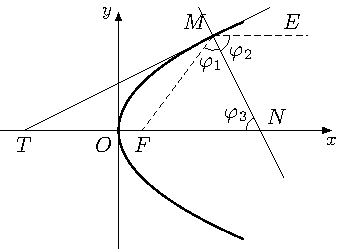
\includegraphics{2-33.pdf}
    \caption{}\label{fig:2-33}
  \end{figurehere}
\end{minipage}

\medskip
\[ y-y_0=-\frac{y_0}{p}(x-x_0).\]
令 $y=0$,便得到法线与 $x$ 轴的交点 $N$ 的坐标 $(x_0+p,0)$,所以
\[|FN|=\left|x_0+p-\frac{p}{2}\right|=x_0+\frac{p}{2}.\]
又由抛物线的定义可知,$|MF|$ 等于点 $M$ 到准线的距离,即
\[|FM|=x_0+\frac{p}{2}.\]
所以
\[|FN|=|FM|.\]
由此得到
\[\varphi_1=\varphi_2.\]

如果点 $M$ 与顶点 $O$ 重合,则法线为 $x$ 轴,结论仍然成立。

将抛物线绕它的对称轴旋转成旋转曲面(旋转抛物面),从\cref{exam:beamer} 我们看到,与对称轴平行的光线投射到曲面上,经曲面反射后便通过焦点。
利用抛物线的这个光学性质可以制作太阳灶(\cref{fig:2-34})。
反过来,放在焦点处的光源发出的光线投射到曲面上,经曲面反射后便成为平行于轴的光线。
利用这个光学性质就可以制作探照灯和汽车前灯(\cref{fig:2-35})等。
\begin{figure}
  \begin{minipage}[b]{0.48\linewidth}\centering
    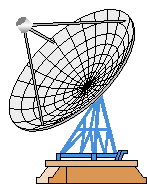
\includegraphics{2-34.pdf}
    \caption{}\label{fig:2-34}
  \end{minipage}
  \begin{minipage}[b]{0.48\linewidth}\centering
    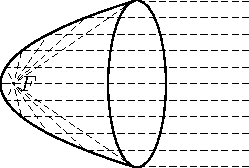
\includegraphics{2-35.pdf}
    \caption{}\label{fig:2-35}
  \end{minipage}
\end{figure}

椭圆和双曲线也有类似的光学性质,不过,在旋转椭圆面的一个焦点发出的光线投射到曲面上,经过曲面反射后,都通过另一个焦点;而在旋转双曲面的一个焦点发出的光线投射到曲面上,经过曲面反射,会使光线散开,而且这些光线就好象是从另一个焦点发出的一样(\cref{fig:2-36})。利用这些性质,可以制造电影放映机上的聚光灯的反射镜面和反射式望远镜中的反射镜等。
\begin{figure}
    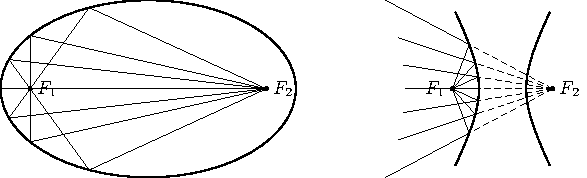
\includegraphics{2-36.pdf}
    \caption{}\label{fig:2-36}
\end{figure}

\begin{Practice}
  \begin{question}
    \item 已知下列曲线上一点的坐标,求在这点的切线和法线方程:
    \begin{tasks}
      \task $y^2-2x=0$,$(18,-6)$;
      \task $9x^2+y^2=25$,$(-1,-4)$;
      \task $\dfrac{x^2}{18}-\dfrac{y^2}{4}=1$,$(6,2)$。
    \end{tasks}
    \item 过点 $P\,(-3,5)$ 作抛物线 $y^2=8x$ 的切线。求切线的方程。
  \end{question}
\end{Practice}
\begin{Exercise}
  \begin{question}
    \item 求下列曲线在已知点的切线的斜率:
    \begin{tasks}(2)
      \task $y^2=10x$,$P\,(3.6,6)$;
      \task $x^2-y^2=1$,$Q\,(2,-\sqrt{3})$。
    \end{tasks}
    \item 求经过点 $P\,(-2,-1)$ 的椭圆 $5x^2+y^2=5$ 的切线方程。
    \item 已知双曲线 $\dfrac{x^2}{10}-\dfrac{y^2}{6}=1$ 的一条切线的斜率等于 2。求这条切线的方程。
    \item 双曲线 $\dfrac{x^2}{4}-\dfrac{y^2}{5}=1$ 的切线平行于直线 $3x-2y=0$,求切线的方程。
    \item $k$ 为何值时,直线 $kx-y-1=0$ 与抛物线 $x^2=4y$
    \begin{tasks}(3)
      \task 相交;
      \task 相切;
      \task 相离?
    \end{tasks}
    \item 已知经过抛物线 $y^2=2px$ 上两点 $P_1\,(x_1,y_1)$ 和 $P_2\,(x_2,y_2)$ 的两条切线相交于点 $M\,(x_0,y_0)$。求证:$x_0=\dfrac{y_1y_2}{2p}$,$y_0=\dfrac{y_1+y_2}{2}$。
    \item 求抛物线 $y^2=9x$ 和圆 $x^2+y^2=36$ 在交点处的切线方程,并求出这两条切线的夹角。
    \item 椭圆 $x^2+4y^2=4$ 的一条切线经过点 $P\,(-\sqrt{2},\dfrac{\sqrt{2}}{2})$,求焦点到这条切线的距离。
    \item 防空探照灯的反射镜与过轴的截面的交线是一条抛物线。已知灯 $\mu$ 直径是 \qty{2000}{mm},深度是 \qty{800}{mm}。光源应放在什么位置?
    \item 有一条光线从抛物线 $y^2=4x$ 的焦点射出,射到抛物线上的点 $P\,(9,6)$,求入射光线和反射光线所在的直线的方程。
  \end{question}
\end{Exercise}
\section*{小结}
\begin{enumerate}[C、,itemindent=4.5em]
  \item 本章在\cref{chp:line}直线方程的基础上,研究了直角坐标系中曲线和方程之间的一一对应关系,然后根据所求曲线的定义,得出了几种圆锥曲线的方程,并通过方程讨论了圆、椭圆、双曲线和抛物线的性质及应用。
  \item 曲线和方程的关系,反映了现实世界空间形式和数量关系之间的某种联系。我们把曲线看作适合某种条件 $p$ 的点 $M$ 的集合
  \[ P = \bigl\{ M \bigm\vert p(M) \bigr\}. \]

  在建立坐标系后,点集 $P$ 中任一元素 $M$ 都有一个有序数对 $(x,y)$ 和它对应,$(x,y)$ 是某个二元方程 $f(x,y)=0$ 的解,也就是说,它是解的集合
  \[ Q = \bigl\{ (x,y) \bigm\vert f(x,y)= 0 \bigr\}\]
  中的一个元素。
  反之,对于解集 $Q$ 中任一元素 $(x,y)$ 都有一点 $M$ 与它对应,点 $M$ 是点集 $P$ 中的一个元素。
  $P$ 和 $Q$ 的这种对应关系就是曲线和方程的关系。
  \item 根据圆的定义,求出了圆的标准方程,又由标准方程推出了圆的一般方程。
  圆的标准方程的优点,在于它明确地指出了圆心和半径,而圆的一般方程则突出了方程形式上的特点,它没有 $xy$ 项,并且 $x^2$、$y^2$ 项的系数相等。
  \item 由椭圆、双曲线、抛物线的几何条件求其标准方程,并通过分析标准方程研究这三种曲线的几何性质。三种曲线的标准方程(各取其中一种)和图形、性质如\cref{tab:2-2}:
  \begin{table}
    \caption{三种曲线的标准方程和图形、性质}\label{tab:2-2}
    \begin{tblr}{colspec={c*3{X[c]}},hline{2}={0.8pt}}
              & 椭圆 & 双曲线 & 抛物线 \\
    几何条件  & 与两个定点的距 离和等于常数 & 与两个定点的距离差 的绝对值等于常数 & 与一个定点和一条 定直线的距离相等 \\
    标准方程  & {$\dfrac{x^2}{a^2}+\dfrac{y^2}{b^2}=1$ \\ $(a>b>0)$}  & {$\dfrac{x^2}{a^2}-\dfrac{y^2}{b^2}=1$ \\ $(a>0,b>0)$}  & {$y^2=2px$ \\ $(p>0)$} \\
    图形  & \begin{minipage}{3.2cm}\centering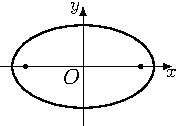
\includegraphics{ellipse.pdf}\end{minipage}  & \begin{minipage}{3.2cm}\centering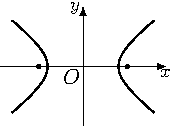
\includegraphics{hyperbola.pdf}\end{minipage}  & \begin{minipage}{3cm}\centering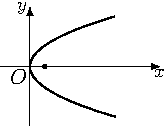
\includegraphics{parabola.pdf}\end{minipage} \\
    顶点坐标  & $(\pm a,0)$,$(0,\pm b)$  & $(\pm a,0)$  & $(0,0)$ \\
    对称轴  & { $x$ 轴。长轴长 $2a$\\ $y$ 轴。短轴长 $2b$} & { $x$ 轴。实轴长 $2a$\\ $y$ 轴。虚轴长 $2b$} & $x$ 轴 \\
    焦点坐标  & {$(\pm c,0)$ \\ $c=\sqrt{a^2-b^2}$} & {$(\pm c,0)$ \\ $c=\sqrt{a^2+b^2}$} & $\left(\dfrac{p}{2},0\right)$ \\
    {离心率 \\$\left(e=\dfrac{c}{a}\right)$}  & $0<e<1$ & $e>1$ & $e=1$ \\
    准线  & $x=\pm\dfrac{a^2}{c}$  & $x=\pm\dfrac{a^2}{c}$ & $x=-\dfrac{p}{2}$ \\
    渐近线  &  & $y=\pm\dfrac{b}{a}x$ &  \\
    \end{tblr}
  \end{table}
  \item 圆、椭圆、双曲线、抛物线的统一性:
  \begin{enumerate}[(1)]
    \item 从方程的形式看: 在直角坐标系中,这几种曲线的方程都是二元二次的,所以把它们称为二次曲线。
    \item 除圆以外,从点的集合(或轨迹)的观点来看: 它们都是与定点和定直线距离的比是常数 $e$ 的点的集合(或轨迹),这个定点是它们的焦点,定直线是它们的准线。只是由于离心率 $e$ 的不同,而分为椭圆、双曲线和抛物线三种曲线。
    \item 从天体运行的轨道看: 天体运动的轨道是这四种曲线,例如,人造卫星、行星、彗星等由于运动的速度的不同,它们的轨道是圆、椭圆、抛物线或双曲线(\cref{fig:2-37})。
    \item 四种曲线又可以看作不同的平面截圆锥面所得到的截线,如\cref{fig:2-38}。因此,它们又统称圆锥曲线。
  \end{enumerate}
  \begin{figure}
    \begin{minipage}[b]{0.48\linewidth}\centering
      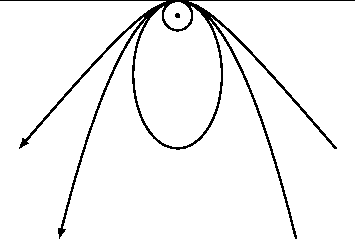
\includegraphics{2-37.pdf}
      \caption{}\label{fig:2-37}
    \end{minipage}
    \begin{minipage}[b]{0.48\linewidth}\centering
      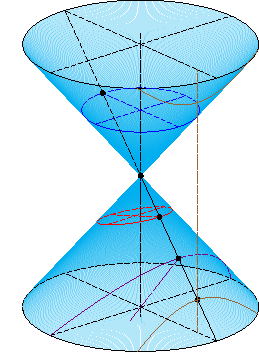
\includegraphics{2-38.pdf}
      \caption{}\label{fig:2-38}
    \end{minipage}
  \end{figure}
  \item 圆锥曲线的切线定义和切线方程的求法,都是初等的。要注意这个方法不完全适用于一般曲线。一般曲线的切线定义和切线方程的求法,将在高中三年级的微积分课程中学习。
\end{enumerate}
\chapter*{复习参考题\chinese{chapter}}
\section*{A 组}
\begin{question}
  \item $A\,(0,7)$、$B\,(1,10)$、$C\,(2,3)$、$D\,(-3,5)$ 四点是否在方程 $3x-y+7=0$ 的直线上?
  \item $A\,(1,-2)$、$B\,(2,-3)$、$C\,(3,10)$ 三点是否在方程 $x^2-xy+2y+1=0$ 的曲线上?
  \item 解答:
  \begin{enumerate}[itemindent=2em]
    \item 求证:在曲线的方程里,如果以 $y$ 代 $x$,同时以 $x$ 代 $y$ 而方程不变,那么曲线关于直线 $y=x$ 对称。
    \item 求证下列方程的曲线关于直线 $y=x$ 对称:
    \begin{tasks}(3)
      \task $xy=k$;
      \task $x^2+y^2=a^2$;
      \task $x^2y+y^2x=k$。
    \end{tasks}
    \item 求证下列各组方程的图形关于直线 $x=y$ 对称:
    \begin{tasks}
      \task $3x+y=1$ 和 $3y+x=1$;
      \task $x^2+(y-a)^2=a^2$ 和 $y^2+(x-a)^2=a^2$;
      \task $y=x^3$ 和 $x=y^3$。
    \end{tasks}
  \end{enumerate}
  \item 点 $M$ 与已知点 $P\,(2,2)$ 连线的斜率是它与点 $Q\,(-2,0)$ 连线的斜率的 2 倍。求点 $M$ 的轨迹方程。
  \item 从一个定点 $M_1\,(a,b)$ 到圆 $x^2+y^2=r^2$ 上任意一点 $Q$ 作线段,$M$ 点内分 $M_1Q$ 成 $2:1$。求点 $M$ 的轨迹的方程。
  \item $\triangle ABC$ 的顶点 $B$、$C$ 的坐标分别是 $(0,0)$、$(a,0)$,$AB$ 边上的中线长为 $m$。求点 $A$ 的轨迹方程。
  \item 如果两条曲线的方程是 $f_1(x,y)=0$ 和 $f_2(x,y)=0$,它们的交点是 $P\,(x_0,y_0)$。证明:方程
\[f_1(x,y)+\lambda f_2(x,y)=0\]
的曲线也经过点 $P$($\lambda$ 是任意实数)。
  \item 从圆 $(x-1)^2+(y-1)^2=1$ 外一点 $P\,(2,3)$,向该圆引切线,求切线的方程。
  \item 求二圆 $x^2+y^2-10x-10y=0$,$x^2+y^2+6x+2y-40=0$ 的公共弦的长。
  \item 在椭圆 $\dfrac{x^2}{45}+\dfrac{y^2}{20}=1$ 上求一点,使它与两个焦点的连线互相垂直。
  \item 由圆 $x^2+y^2=4$ 上任意一点,向 $x$ 轴作垂线。求垂线夹在圆周和 $x$ 轴间的线段中点的轨迹方程。
  \item \label{exec:2t-12} 如图,从椭圆上一点 $P$ 向 $x$ 轴作垂线,恰好通过椭圆的一个焦点,这时椭圆的长轴的端点 $A$ 和短轴的端点 $B$ 的连线平行于 $OP$。求椭圆的离心率。
  \begin{figurehere}
    \begin{minipage}{\linewidth}\centering
      \includegraphics{2t-12.pdf}
      \caption*{(第 \ref{exec:2t-12} 题)}
    \end{minipage}
  \end{figurehere}
  \item 已知中心在原点的双曲线的一个焦点是 $F_1\,(-4,0)$,一条渐近线的方程是 $3x-2y=0$。求双曲线的方程。
  \item 已知双曲线的离心率为 2,求它的两条渐近线的夹角。
  \item 一个圆的圆心在双曲线 $x^2-3y^2=12$ 的右焦点上,并且该圆过原点。求这个圆和双曲线的交点的坐标。
  \item 已知抛物线的顶点在原点,焦点在 $x$ 轴上,并且经过点 $Q\,\left(\frac{3}{2},-4\right)$。求它的方程。
  \item 解答:
  \begin{tasks}
    \task 从抛物线 $y^2=2px$ 上各点,作 $x$ 轴的垂线段,求线段中点的轨迹;
    \task 求抛物线 $y^2=2px$ 上各点与焦点连线中点的轨迹。
  \end{tasks}
  \item 设抛物线的顶点为 $O$,经过焦点垂直于轴的直线和抛物线交于两点 $B$、$C$,经过抛物线上一点 $P$ 垂直于轴的直线和轴交于点 $Q$。求证:线段 $|PQ|$ 是 $|BC|$ 和 $|OQ|$ 的比例中项。
  \item 从抛物线的焦点向它的任一切线引垂线,求证:这条垂线和准线的交点在过切点且平行于对称轴的直线上。
  \item 过抛物线焦点的直线与抛物线相交于两点,求证:抛物线在这两点的切线互相垂直。
  \item $k$ 为何值时,直线 $y = {kx}$ 与双曲线 $4x^2 - y^2 = {16}$,
  \begin{tasks}(3)
    \task 相交;
    \task 相离;
    \task 能相切吗?为什么?
  \end{tasks} 
  \item 求抛物线 $y=x^2$ 上到直线 $y=2x-4$ 的距离最小的点的坐标,并求出这个距离。
\end{question}
\section*{B 组}
\begin{question}[resume]
  \item 底面直径为 \qty{12}{cm} 的圆柱被与底面成 \ang{30} 角的平面所截,截口是一个椭圆。求这个椭圆的方程。
  \item 过圆外一点 $P\,(a,b)$,引圆 $x^2+y^2=R^2$ 的两条切线。求经过两个切点的直线方程。
  \item 已知二定点 $A\,(-1,0)$、$B\,(2,0)$,求使得 $\angle MBA= 2\angle MAB$ 的点 $M$ 的轨迹方程。
  \item 设 $A_1$、$A_2$ 是一个圆的一条直径的两个端点,$P_1P_2$ 是与 $A_1A_2$ 垂直的弦,求直线 $A_1P_1$ 与 $A_2P_2$ 交点的轨迹方程。
  \item 设直线 $y=(1-x)\tan\alpha$ 与双曲线 $-x^2+y^2\cos^2\alpha=1$ 相切,求 $\alpha$ 的值及切点坐标。
  \item 求证: 直线 $y=kx+m$($m\neq 0$)与椭圆 $\dfrac{x^2}{a^2}+\dfrac{y^2}{b^2}=1$、双曲线 $\dfrac{x^2}{a^2}-\dfrac{y^2}{b^2}=1$、抛物线 $y^2=2px$ 相切的充要条件分别是 $k^2a^2+b^2=m^2$,$k^2a^2-b^2=m^2$,$k=\dfrac{p}{2m}$。
  \item 点 $P$ 与两定点 $F_1\,(-a,0)$、$F_2\,(a,0)$ 连线的斜率的乘积是常数 $k$,求点 $P$ 的轨迹方程。讨论当 $k$ 的值变化时,轨迹都是什么曲线,并在同一坐标系中画出它们的图形。
\end{question}